\pdfoutput=1 
\documentclass[a4paper,12pt]{article}

\usepackage{graphicx}% Include figure files



\graphicspath{{./Figures/}}
% packages
\usepackage{comment}
\usepackage{amsfonts}
\usepackage[dvipsnames]{xcolor}
\usepackage{placeins}
\usepackage[perpage]{footmisc}
\usepackage[normalem]{ulem}
\usepackage{caption}
\usepackage{makecell}
\usepackage{subcaption}
%\usepackage{subfig}
\usepackage{jinstpub} 
\usepackage{multicol,tabularx,capt-of}
\usepackage{hhline}
\usepackage{booktabs}
\usepackage{multirow}
\usepackage{lineno}
\usepackage{xfrac}
\usepackage{url}
\usepackage{soul}
\usepackage{hyperref}
\usepackage{chemformula}

\usepackage[binary-units,separate-uncertainty=true]{siunitx}
\usepackage{mathtools} 
%\usepackage{amssymb}
\usepackage{physics}
\usepackage[colorinlistoftodos, textsize=tiny, obeyFinal]{todonotes}



\newcommand{\DR}{DR8}
\newcommand{\RI}[1]{\textcolor{blue}{#1}}
\newcommand{\quotes}[1]{``{#1}''}


\title{Carbon-Loaded Kapton as an Electric Field Shaping Material, a Novel Approach for Time Projection Chambers}

\author[a,1]{J.Doe,\note{Corresponding author}}


\affiliation[a]{SLAC National Accelerator Laboratory,\\ Sand Hill Rd. Menlo Park, Ca, 94025, USA}
\affiliation[b]{Michigan State University,\\ 426 Auditorium Rd. East Lansing, Mi, 48824, USA}


\abstract{Conventional liquid noble gas time projection chambers (TPCs) consist of discreet field-shaping rings between a cathode and an anode, to maintain a uniform electric field throughout the drift volume. 
	The field-shaping rings are connected by a resistor chain to gradually reduce the voltage, approximating a linear potential gradient. 
	Here, we present a novel alternative approach to field shaping using a continuous resistive plane formed of {\DR}. 
	{\DR} is a highly resistive carbon-loaded Kapton foil ($\order{10~\mathrm{G}\Omega\,\mathrm{sq}^{-1}}$ at room temperature and low electric field.
	We report studies of the electrical properties of {\DR} performed in several apparatus. 
	We find that the resistance dependence is exponential with the square root of the temperature, resulting in an increase in the resistivity of {\DR} by an order of magnitude when cooled to \SIrange{77}{90}{\kelvin}. 
	We also find that the dependence on the applied voltage follows the hopping-transportation model, with an exponential decay with respect to the square root of the electric field.} 



\keywords{Cryogenic detectors}

\begin{document}
\listoftodos
\maketitle

\todo{implement new structure}
\begin{comment}
	
	\section{Introduction} and concept of resistive sheet
	Concept of resistive sheet
	Possible physics applications -> requirements (which motivate the measurements we did)
	\section{Methodology}
	Fabrication of resistive sheet
	Test stands
	\section{Results}
	Voltage dependance
	Temperature dependance - includes LN temperature
	Surface area of contact overlap
	Transmission line measurement - Dan did this, estimate of contact resistance
	Aging measurement - Not in the paper yet - to be prepared, needs Zach
	=> Francois will clean up results section except for aging
	=> Francois, who else do we need and what specific figure edit needs to happen?
	\section{Discussion  and conclusions} 
	Suitability of applications
	
\end{comment}



\section{Introduction}
\label{sec:intro}
\subsection{Motivation}
The use of time projection chambers (TPC) has increased significantly over the past decades, particularly in the fields of neutrino physics~\cite{Acciarri:2016ooe,Adams:2019bzt,Amerio:2004ze}, direct detection of dark matter~\cite{Aprile:2012zx,Akerib:2019fml,Aalseth:2017fik} and neutrino-less double beta-decay~\cite{Pocar:2020zqz}. 
The main advantage of TPCs is that they offer an active volume that is simultaneously a tracking and a calorimetric detector.

Most experiments in the aforementioned fields utilize argon or xenon, in either gaseous or liquid form, as the detection medium. 
The TPC relies on the deposition of energy by charged particles passing through the detector. 
Much of this energy converts atoms in the volume into charged pairs of electrons and ions. 
These electrons are then drifted by a uniform electric field to a readout plane at the anode, where they are detected. 
The ionization process also produces scintillation light which is collected by photo sensors. 
These two signals are combined to reconstruct detailed three dimensional images of particle interactions.

The electric field is generated by applying a bias voltage to the cathode and using a resistor chain to drop the voltage to ground at the anode.  
Electric-field uniformity is achieved by connecting conducting field-shaping ``rings'' at the junction between each resistor in the chain, We refer to the field-shaping rings collectively as the ``field cage''. 
The value of the resistors is chosen based on the current draw that the system can handle.
This design has been employed in TPCs since their inception with very little change despite some non-negligible drawbacks. 

TPCs are essentially parallel plate capacitors that store energy as a function of applied voltage and volume. 
For small TPC this is not an issue as short drift distances require low cathode voltages.
However, for kilotonne-scale TPCs like the DUNE far detectors the stored energy is $\order{\SI{100}{\joule}}$~\cite{Acciarri:2016ooe}.
This issue is compounded by the use of metal in traditional field cages, if a ring is allowed to short to ground the energy at that point in the TPC will be dumped instantaneously. 
The DUNE collaboration investigated the use of a resistive cathode~\cite{DUNE:2017pqt} to reduce the energy release rate in the case of a discharge.
To prevent discharges from the metallic field cage to the cryostat or pressure vessel, clearance volumes set by the dielectric strength of the target material are used. 
In the case of liquid argon, the dielectric strength is only \SI{40}{\kilo\volt\per\centi\metre}~\cite{MicroBooNE:2014php}, which leads to nearly \SI{7}{\kilo\tonne} of un-instrumented argon per DUNE far detector cryostat~\cite{Acciarri:2016ooe}.
Neglecting the cost of purchasing, purifying, and cooling the target material, un-instrumented mass is not desirable in any statistics-limited experiment.        
There are methods to mitigate discharges~\cite{Auger:2014eba}, but is safer to avoid very high electric fields.  
The ArgonCube collaboration proposed to segment the TPC, reducing the required electric field, and using copper-on-fiberglass printed circuit board technology to produce the TPC~\cite{Auger:2268439}. 
Fiberglass has a dielectric strength of \SI{200}{\kilo\volt\per\centi\metre}~\cite{5071132}, which allows the clearance volumes to be negated.
The Bern group built on the DUNE resistive cathode concept and used {\DR} in place of a resistor chain and field cage to produce a TPC with continuous electric field shaping~\cite{bern_lartpc}.   

Here, we build on Bern's efforts in characterizing {\DR} as an electric field shaping technology for cryogenic noble gas TPCs.
We present several apparatus aimed at quantifying the properties of {\DR} by characterizing its resistive behavior under different regimes, which in practice consists of monitoring the current accurately at a given voltage and temperature. 
In addition we demonstrate a technique for manufacturing a TPC utilizing {\DR}.

\subsection{Charge Transportation in Disordered Material}
\label{sec:disorder_Mattrial}

{\DR}, is a carbon-loaded Kapton\footnote{DuPont\texttrademark, Kapton\textregistered \, polyimide film, E. I. du Pont de Nemours and Company, \url{www.dupont.com}.} foil ($\sim$~\SI{100}{\micro\metre}). 
Its electrical properties are expected to follow disordered system properties. 
The resistance of a given material $R$ depends on its geometry, and is described by the following equation:
\begin{equation}
\label{eq:Res_3D}
R \equiv \rho \frac{L}{S} \ [\Omega],
\end{equation}

where $L$ is the length of the resistive material along the current direction, $S = W \cdot T$ is its cross-sectional area, and $\rho$ is the intrinsic resistivity of the material. 
For thin films (such as {\DR}), the thickness $T$ of the sheets is considered negligible, and instead, the intrinsic characteristic is taken to be the \emph{sheet resistance} $R_s$ and is defined:
\begin{equation}
\label{eq:res_2D}
R_s \equiv \rho \frac{W}{L} \ [\Omega / \Box],
\end{equation}
where $W$ is the width of the material perpendicular to the current direction. 
Note that the units for sheet resistance are ``Ohms per square'' ($\Omega / \Box$), yet the physical dimension of sheet resistance is the same as that of usual resistance. 
The $\Box$ denotes that the resistance measurements correspond to a sheet resistance rather than the usual bulk resistance.

The electrical resistivity (conductivity) properties of disordered organic materials are rich and quite different to regular resistors. 
These materials are usually described as a network of conducting sites embedded within an insulator. 
Electrons at each ``node'' of the network are bounded under a potential well and can be transported via tunneling to other nodes. 
This is sometimes described by Percolation theory~\cite{Havlin1996} and is referred to as \emph{Hopping-Transportation}, for detailed description see~\cite{organicDisorderMaterial,electronicPhotonicMaterials}.

Specifically, the resistivity of these materials depends on the applied electric field and temperature.  
In high electric fields, the charge carrier transport coefficient increases with the field strength, being approximately proportional to $e^{\sqrt{E/E_0}}$, where $E$ is the electric field applied. 
In terms of resistivity this can be re-written as:

\begin{equation}
\label{eq:efield}
{R_s} \propto e^{- (E / E_0)^{1/2}},
\end{equation}

The temperature dependence follows

\begin{equation}
\label{eq:Tdep}
R_s \propto  e^{( \Delta(T) / k_B T)^{\beta}},
\end{equation}

where $T$ is the temperature, $k_B$ is the Boltzmann constant, $\Delta(T)$ is the activation energy, and $\beta$ is an exponent which depends on the specific material.
Both the temperature and electric-field dependence will be characterized in the following sections.  


\section{Methodology}
\label{sec:expsetup}

 
Three test stands we used for characterizing {\DR}; two at SLAC and one at Michigan State University (MSU).
The larger of the two SLAC test stands, shown in Figure~\ref{fig:full_sys}, is used for long-term measurements in liquid argon.    
The smaller SLAC test stand, shown in Figure~\ref{fig:slac_styro_setup}, was used for initial measurements and validation of prototypes in liquid nitrogen. 
The MSU test stand is shown in Figure~\ref{fig:msu_styro_setup}, it was used to characterize construction parameters of the {\DR} samples and for the transmission line measurements.  


\subsection{Liquid argon test stand}

\begin{figure}[ht]
	{\includegraphics[width=0.6\linewidth]{inside_rans.jpg}}
	{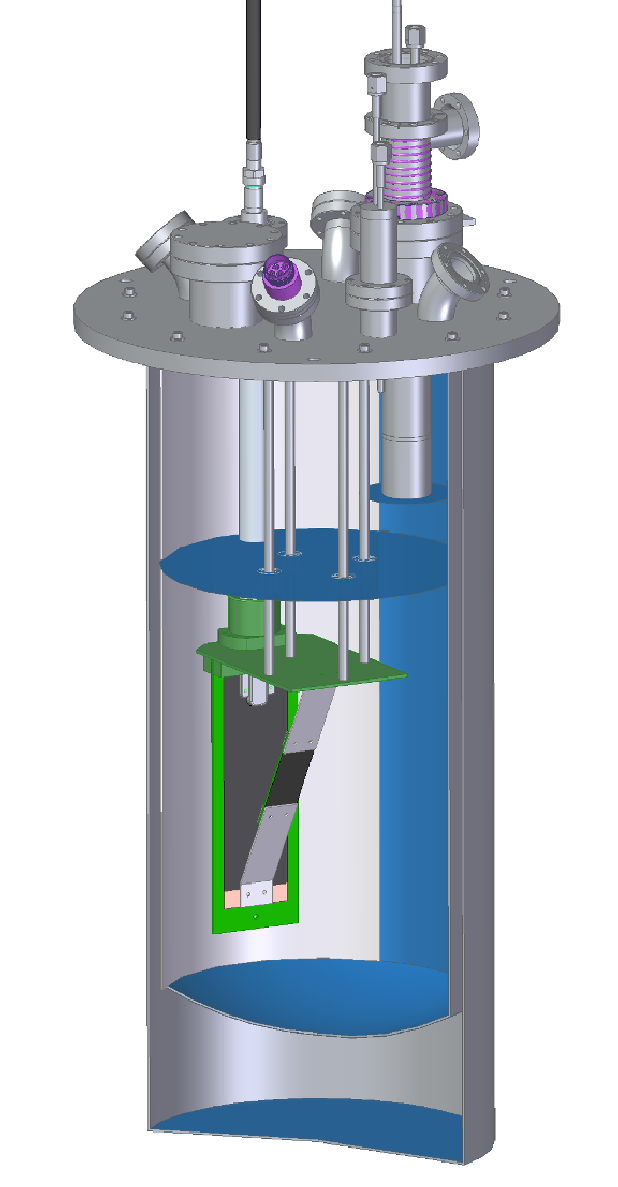
\includegraphics[width=0.42\linewidth]{rans.png}}
	\caption{(Left) A photograph of the liquid argon test assembly.
		The white tube is a polytetrafluoroethylene dielectric shield for the high voltage feedthrough that connects to a stainless port in the top of the dummy cathode. 
		The {\DR} sample is mounted at an angle between the base of the cathode and a ground point on the fiber glass support structure. 
		The cathode resistance is four orders of magnitude lower than the {\DR} sample.
		(Right) A CAD of the liquid argon test stand. 
		The blue surface is the liquid level. 
		The cylinder on the right is a thermosyphon used to provide cooling.}
	\label{fig:full_sys}
\end{figure}

The system, shown in Figure~\ref{fig:full_sys}, is a \SI{65}{\litre} vacuum-jacketed cryostat which is filled with liquid argon. 
is designed to achieve stable cryogenic conditions for periods of multiple months. 


For long term operation, cooling is provided by a liquid nitrogen thermosyphon of the type developed for LUX~\cite{lux}.
The temperature is maintained between \SIrange{89}{92}{\kelvin} at an accuracy of \SI{0.1}{\kelvin}. 
This is achieved with control loop using a heater to mitigate freezing at the there thermosyphon and an array of PT100 Resistance Temperature Detectors (RTDs).
The temperature is logged throughout data taking.   

The high voltage (HV) feedthrough utilizes the nEXO design~\cite{nEXO_pcdr}, as also adopted by DUNE~\cite{DUNE:2021tad}. 
The feedthrough is designed for \SI{150}{\kilo\volt}, but the voltage in this application is limited by the power supply~\footnote{Glassman FR50R6} to \SI{50}{\kilo\volt}. 

describe HV probe. 


It consists of a system connecting in series a High Volatage (HV) cable, a cathode made out of resistive Kapton XC~\footnote{DuPont High-Performance Materials}, a {\DR} sample, and a ground return line. 


The testing assembly can be thought of as a partial TPC with the HV feedthrough terminating at a cathode that connects to a ground return via a sample of field-shaping material. 
Here, {\DR} is used as the field-shaping, but any resistive material can be tested in this assembly.    
The structure of the assembly is FR4, chosen for its dielectric strength and cryogenic compatibility.
All electrical connections are made with stainless-steel brackets. 
The cathode consists of a sheet of FR4 with a conductive Kapton foil laminated to it.   
The \numproduct{15 x 15}~\unit{\centi\metre\squared} {\DR} sample is metallized section of FR4 with {\DR} laminated to it.
The lamination process is explained in section~\ref{sec:lamination}.
At these dimensions, the {\DR} samples requires a cathode voltage of \SI{12.5}{\kilo\volt} to achieve a field of \SI{1}{\kilo\volt\per\centi\metre}.    

The data acquisition (DAQ) monitors the current running through the sample with a picoammeter~\footnote{Keithley 6485} connected in series with the \DR sample in the path of the HV ground. 
A gas discharge tube is connected in parallel to the picoammeter to protect it from high voltage discharges. 
The voltage is measured by the internal voltage monitor of the power supply.
\todo{circuit diagram, fix caption}

\begin{figure}[ht]
	{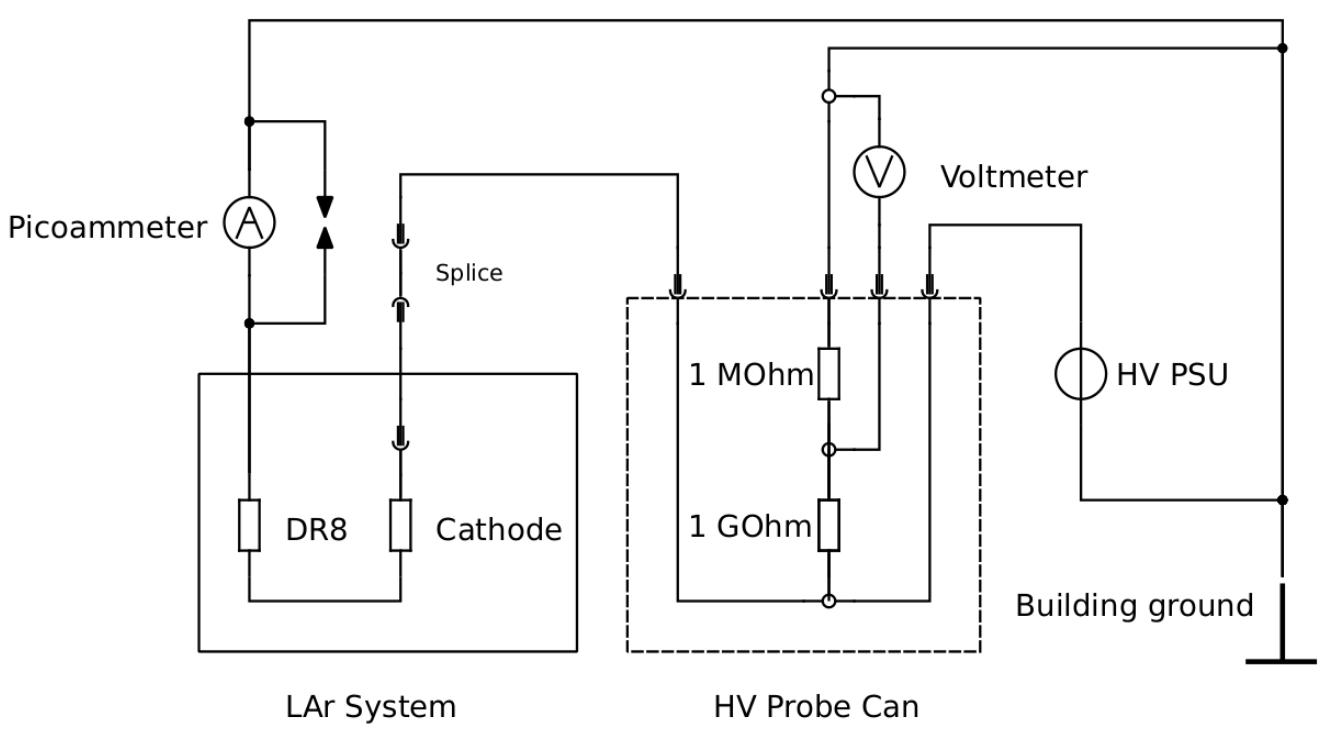
\includegraphics[width=0.85\linewidth]{circuit.jpg}}
	\caption{circuit diagram of the long-term test stand. the voltage is measure via a potential divider, the current is measured using  picoammeter in the ground path. }
	\label{fig:circuit}
\end{figure}
\todo{confirm values of divider}

The DAQ software consists of a simple Dash\footnote{\href{https://plotly.com/dash/}{https://plotly.com/dash/}}-based GUI\footnote{\href{https://github.com/francois-drielsma/kapton_daq}{https://github.com/francois-drielsma/kapton\_daq}} driving the InstrumentKit\footnote{\href{https://github.com/Galvant/InstrumentKit}{https://github.com/Galvant/InstrumentKit}} API as a back-end. 
The software periodically queries the picoammeter and the power supply. 
The picoammeter returns a string at each query which provides a seven-digit signed mantissa and a power of 10 exponent. 
The power supply returns an unsigned 10-bit hex string for the voltage. 
The string divides the full voltage range from \SIrange{0}{50}{\kilo\volt} (3FF) in 1024 steps of $\sim$~\SI{50}{\volt}, limiting the system's resolution. The query speed limits the acquisition rate to $\sim$~\SI{10}{\hertz}.


\todo{NOT CHECKED YET Details on Lamination - NO mention of DUNE!! not a word.}

\todo{NOT CHECKED YET Kill all alternative design, this is a tech paper not DoE politics.} 


\subsection{SLAC liquid nitrogen test stand}


A schematic of the SLAC secondary system is shown in Figure~\ref{fig:slac_styro_setup}. It is built around an off-the-shelf cooler box, which provides sufficient insulation to hold $\mathcal{O}(10)$\,liters of cryogen for periods of a few hours. The walls and the lid of the box consist of $\sim5$\,cm of expanded polystyrene foam (EPS) with inner dimensions of $\sim30\times60\times30$\,cm$^3$. The lid is modified by adding a $\sim5$\,cm layer of extruded polystyrene foam (XPS), a $\sim20$\,cm XPS chimney and a removable windowed port. Several holes are drilled to accommodate the high voltage cable, a ground line, the high voltage probe and a cryogen funnel.

\begin{figure}[htb]
\centering
\begin{subfigure}[c]{0.49\linewidth}
	\begin{center}
		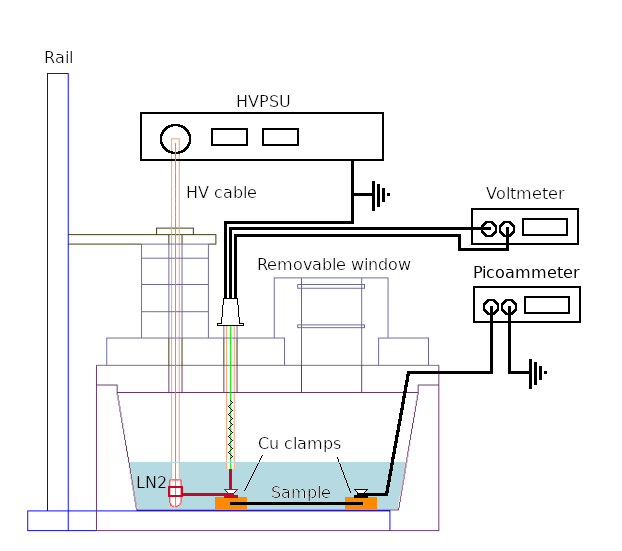
\includegraphics[width=\linewidth]{slac_styro_setup.png}
		(a)
	\end{center}
\end{subfigure}
\begin{subfigure}[c]{0.49\linewidth}
	\begin{center}
		\vspace*{1em}
		
		\includegraphics[width=\linewidth]{slac_styro_setup_picture.png}
		\vspace*{0.5em}
		
		(b)
	\end{center}
\end{subfigure}
\caption{(a) Schematics and (b) picture of the secondary apparatus operated at SLAC.}
\label{fig:slac_styro_setup}
\end{figure}

\todo{fix text significant overlap, put description in previous section.}
The high voltage delivery is very similar to the main system and uses the same resistive-core high voltage cable. A Glassman FR50N6 power supply provides up to 50\,kV/6\,mA of DC voltage.  A flange holds the cable in place using an 80/20 stand fitted with a Delrin plate. The cold side of the cable is shielded by XPS chimney and its exposed end is submerged in $\sim10$\,cm of cryogen. The conductive pill is connected to the one edge of the sample under test by an 18 AWG wire attached to the pill with a hose clamp and to the sample with an alligator clip.

The voltage is monitored with a commercial 40\,kV high voltage probe, i.e. a 1:1000 voltage divider composed of one 1\,G$\Omega$ and one 1\,M$\Omega$ resistors connected in series. A Keithley DMM6500 digital multimeter is connected in parallel to the 1\,M$\Omega$ resitor and measures the scaled DC voltage upstream of the sample. It achieves an absolute voltage resolution of $\mathcal{O}(1)\,$V.

The current running through the sample is monitored in series with a Keithley 6485 picoammeter which is sensitive to currents as low as 10\,pA. It is connected to the ground side of the sample on one end and to the building ground on the other. A gas discharge tube is connected in parallel of the picoammeter in order to protect it from discharges. The current flow bypasses the picoammeter if the voltage across it exceeds 10\,V.

Two classes of samples are tested. Loose sheets of DR8 are clamped on both sides with two pairs of copper bars pressed together with thumb screws. Laminated samples that are not copper clad are metalized with conductive-adhesive copper tape. Both of them are connected on either side with an alligator clip. The samples can be tested both at room temperature and completely submerged in liquid nitrogen. No test was conducted using liquid argon in this system. The temperature is monitored with a K-type thermocouple placed nearby the ground side of the sample. The thermocouple is read out with Fluke t3000 FC wireless temperature module.

\subsubsection{MSU liquid nitrogen test stand}
\label{sec:MSU}

\todo{eliminate any redundancy with previous section}

A diagram of the MSU test stand is shown in Figure~\ref{fig:msu_styro_setup}.  Similar to the SLAC apparatus, the main testing chamber is a re-purposed EPS cooler box with inner dimensions of $\sim 15 \times 20 \times 10\,$cm$^3$, for a total capacity of $\sim 3.2\,$ L.  The walls of the chamber are of a similar thickness to the SLAC apparatus, $\sim 5\,$ cm, which provides for several hours of operation with little cryogen evaporation.  Feedthrough of high-voltage power is achieved by a square aluminum panel mounted over a small cutout in the chamber lid.  This panel features an SHV connector for the power supply side and a BNC connector for the low-voltage return side.  Internally, the connectors interface with two Polytetrafluoroethylene (PTFE) insulated conductors, each connected to a copper clamp for contacting the sample.  The high voltage delivery system for this apparatus does not feature a resistive-core cable and pill assembly for HV delivery as in the other two systems.

High voltage power is supplied by a Bertan model 5900 HVPS.  This unit is connected directly to the input connection of the testing chamber.  Inside, the high voltage line is connected to a 40 kV high voltage probe, a 1:1000 voltage divider identical to the one used in the SLAC secondary apparatus.  At this point, the high voltage line is also connected to one end of the sample under test via copper clamps.  The other end of the sample is then connected to the return BNC line, which in turn connects to a Kiethley 2000 multimeter.

The return path is completed through the outer conductor of the BNC cables, which is tied to ground at the meter, the chamber panel, and the power supply and its housing.

The multimeter is used for measuring both the current through the sample and the voltage probe, and is controlled remotely via computer over a serial interface.  This meter has a resolution of 10 nA, and so samples for testing in this chamber are designed with a much wider aspect ratio than those used in the SLAC system, meaning a relatively shorter distance between contacts.  This allows for greater currents through the samples, as well as the ability to reach higher field strengths with lower voltage.

\begin{figure}[htb]
\centering
\begin{subfigure}[c]{0.59\linewidth}
	\begin{center}
		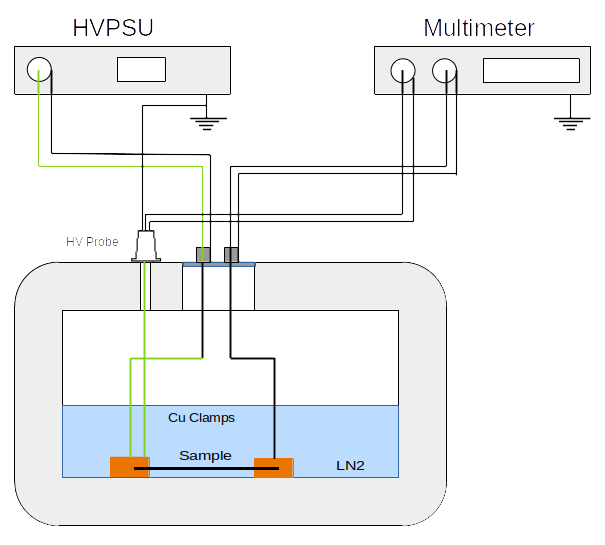
\includegraphics[width=\linewidth]{MSU_styro_setup.png}
		(a)
	\end{center}
\end{subfigure}
\begin{subfigure}[c]{0.39\linewidth}
	\begin{center}
		\vspace*{4em} 
		
		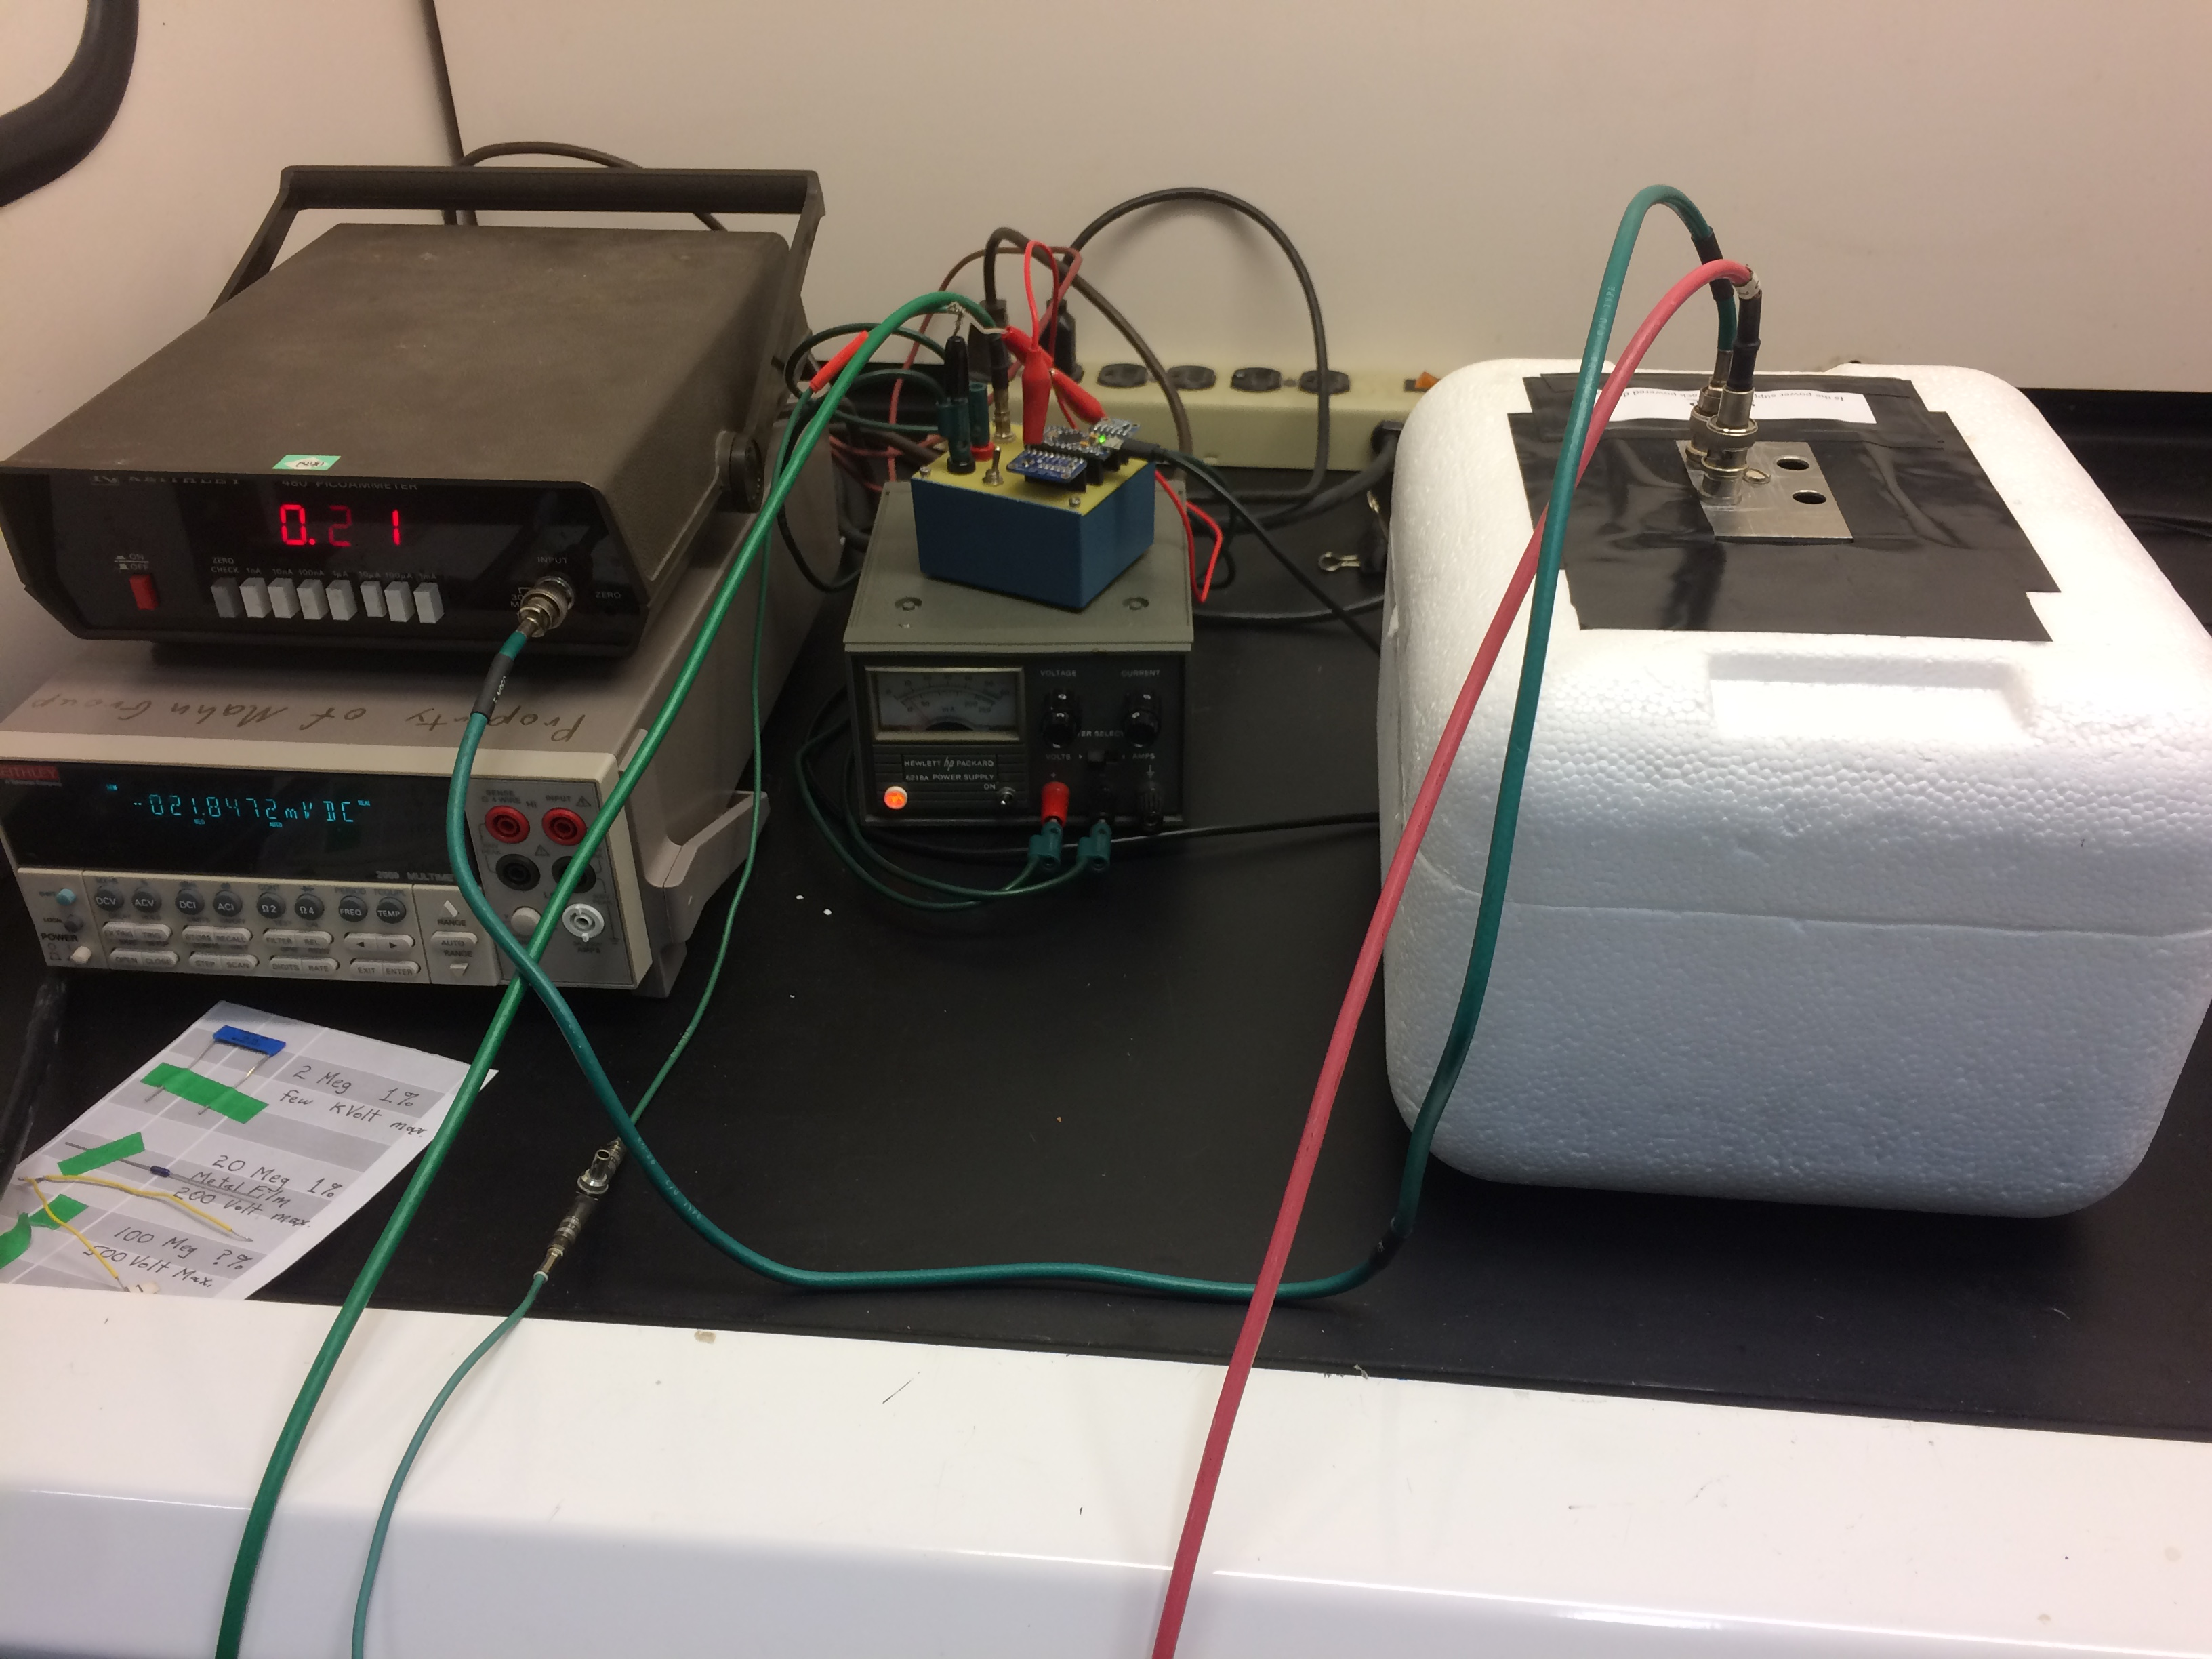
\includegraphics[width=\linewidth]{MSU_styro_setup_picture.jpg}
		\vspace*{3em} 
		
		(b)
	\end{center}
\end{subfigure}
\caption{Schematic representation (a) and photograph (b) of the secondary apparatus operated at MSU.}
\label{fig:msu_styro_setup}
\end{figure}


\subsection{DR8 Sample production}
\label{sec:field_shell}
\textcolor{blue}{Francois}

The material studies conducted on Kapton DR8 in this paper are performed with the intention of evaluating its viability in a field shell, i.e. a field-shaping structure which uses continuously resistive sheets to smoothly decrease the voltage. This approach to field-shaping has several key advantages over a traditional TPC field cage:

\todo{move following to the introduction. if not repetition}
\begin{itemize}
\item It extends the achievable active volume by having a smaller footprint and also by reducing local field non-uniformity created by field-shaping rings;
\item The resistive heating is spread over entire panels instead of being localized on the surface of resistors, which drastically stifles liquid argon nucleation;
\item It does not suffer from single points of failure, as the whole panel drives the resistance;
\item The field does not spike around rings, considerably reducing the risk of arcing.
\end{itemize}

This section summarizes the field shell designs studied in the context of this paper and the techniques developed to make them feasible.

\subsection{Designs}
Previous prototypes~\cite{bern_lartpc,srmu_tpc} used frames on which the resistive material was attached. Figure~\ref{fig:field_shell} shows schematics of the baseline DUNE-ND field-shaping design as a whole. It is composed of five copper-clad FR4 panels covered with electroconductive Kapton sheets. The central panel in the figure is the cathode -- which splits the TPC module into two drift volumes and sets the maximum potential -- while the other four form the `field shell': a resistive structure which continuously decreases the voltage from the cathode to the grounded anode. The field-shaping structure also provides mechanical support for the entire TPC module and optically isolates it from adjacent modules.
\todo{add single cube figure, drawing and pictures}


\todo{Francois: Add text about material for field shell and replace this figure with a picture of SLAC single cube}

The cathode panel is covered on both sides with a layer of 25\,$\mu$m-thick Kapton XC, a material which provides a $\mathcal{O}(1)\,$M$\Omega/\Box$ sheet resistance, identical to the one used in the protoDUNE-SP cathode~\cite{protodune_sp_tdr}. It is not subject to further study in this paper. The field shell panels are covered with 100\,$\mu$m-thick sheets of {\DR}, a variant of Kapton XC which exhibits a higher $\mathcal{O}(1)\,$G$\Omega/\Box$ sheet resistance at room temperature and under low voltage loads \RI{ Francois, should we change to e-fields, as this is our claim?}. This material is a suitable basis to replace traditional field cages as it provides sufficient bulk resistance to constrain the heat load and limit the necessary power supply power. The properties of {\DR} are extensively studied in this paper.


Figure~\ref{fig:shell_designs} shows the three possible shell configurations under consideration. The \textit{full} design corresponds to the baseline, the \textit{zebra} design reduces the Kapton coverage by connecting the anode and cathode with a series of parallel {\DR} strips of fixed width and the \textit{ladder} design steps the voltage discretely between successive copper bands connected by a few strips of {\DR}. The last two designs have the advantage of reducing the amount of {\DR} needed in each field shell, reducing the cost of the manufacturing and increasing the bulk resistance of the shell, thus reducing the resistive heat load. Their electrical properties are briefly investigated in this paper.

\begin{comment}
	content...

\begin{figure}[htbp]
\centering

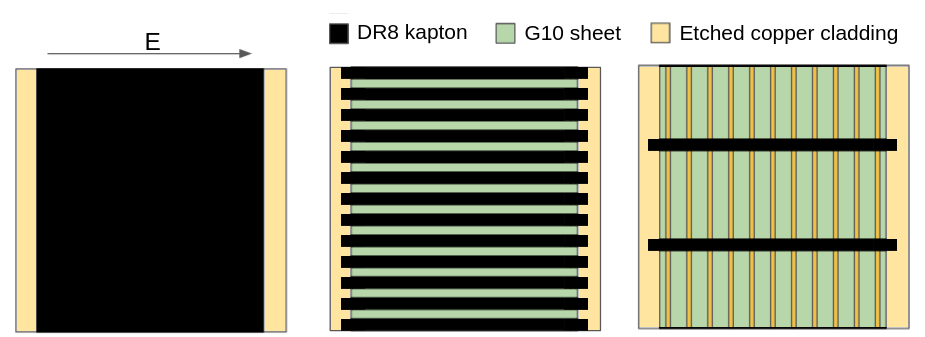
\includegraphics[width=.9\linewidth]{shell_designs_noccc.png} \\
(a) \hspace{0.25\textwidth} (b) \hspace{0.25\textwidth} (c)
\caption{Field shell designs under study: (a) full, (b) zebra and (c) ladder.}
\label{fig:shell_designs}
\end{figure}
\end{comment}
\todo{Francois? removed figure 6, adjust text since Figure 7 will show it}


\subsection{Lamination}
\label{sec:lamination}
In order to build field shell panels, a method to laminate the conductive Kapton onto the copper-clad FR4 panels was demonstrated. It employs a purpose-built lamination device or \textit{laminator} (Figure~\ref{fig:field_shell_laminations}a), and follows these steps:
\begin{enumerate}
\item Etch copper-clad FR4 panels leaving only a 1.25\,cm-thick bands of copper on the cathode and anode sides;
\item Laminate a sheet of protective plastic on the back of the panel, mask part of the copper bands with tape to prevent epoxy from getting on them;
\item Tape Kapton sheets or strips in the desired pattern onto the laminator table, laminate them with protective film, lift the film off the table;
\item Apply $250$\,g/m$^2$ of epoxy\footnote{Master Bond EP29LPSP} on the FR4 panel, roll {\DR} onto the glue, ensure $>5\,$mm overlap with each copper band;
\item Cover the laminate with bleeder cloth, vacuum bag the assembly, cure for seven days at room temperature, with the first two days under vacuum.
\end{enumerate}
Three small panels produced using this method are shown on Figure~\ref{fig:field_shell_laminations}b.

\begin{figure}[htbp]
\centering
\begin{subfigure}[c]{0.3575\linewidth}
	\begin{center}
		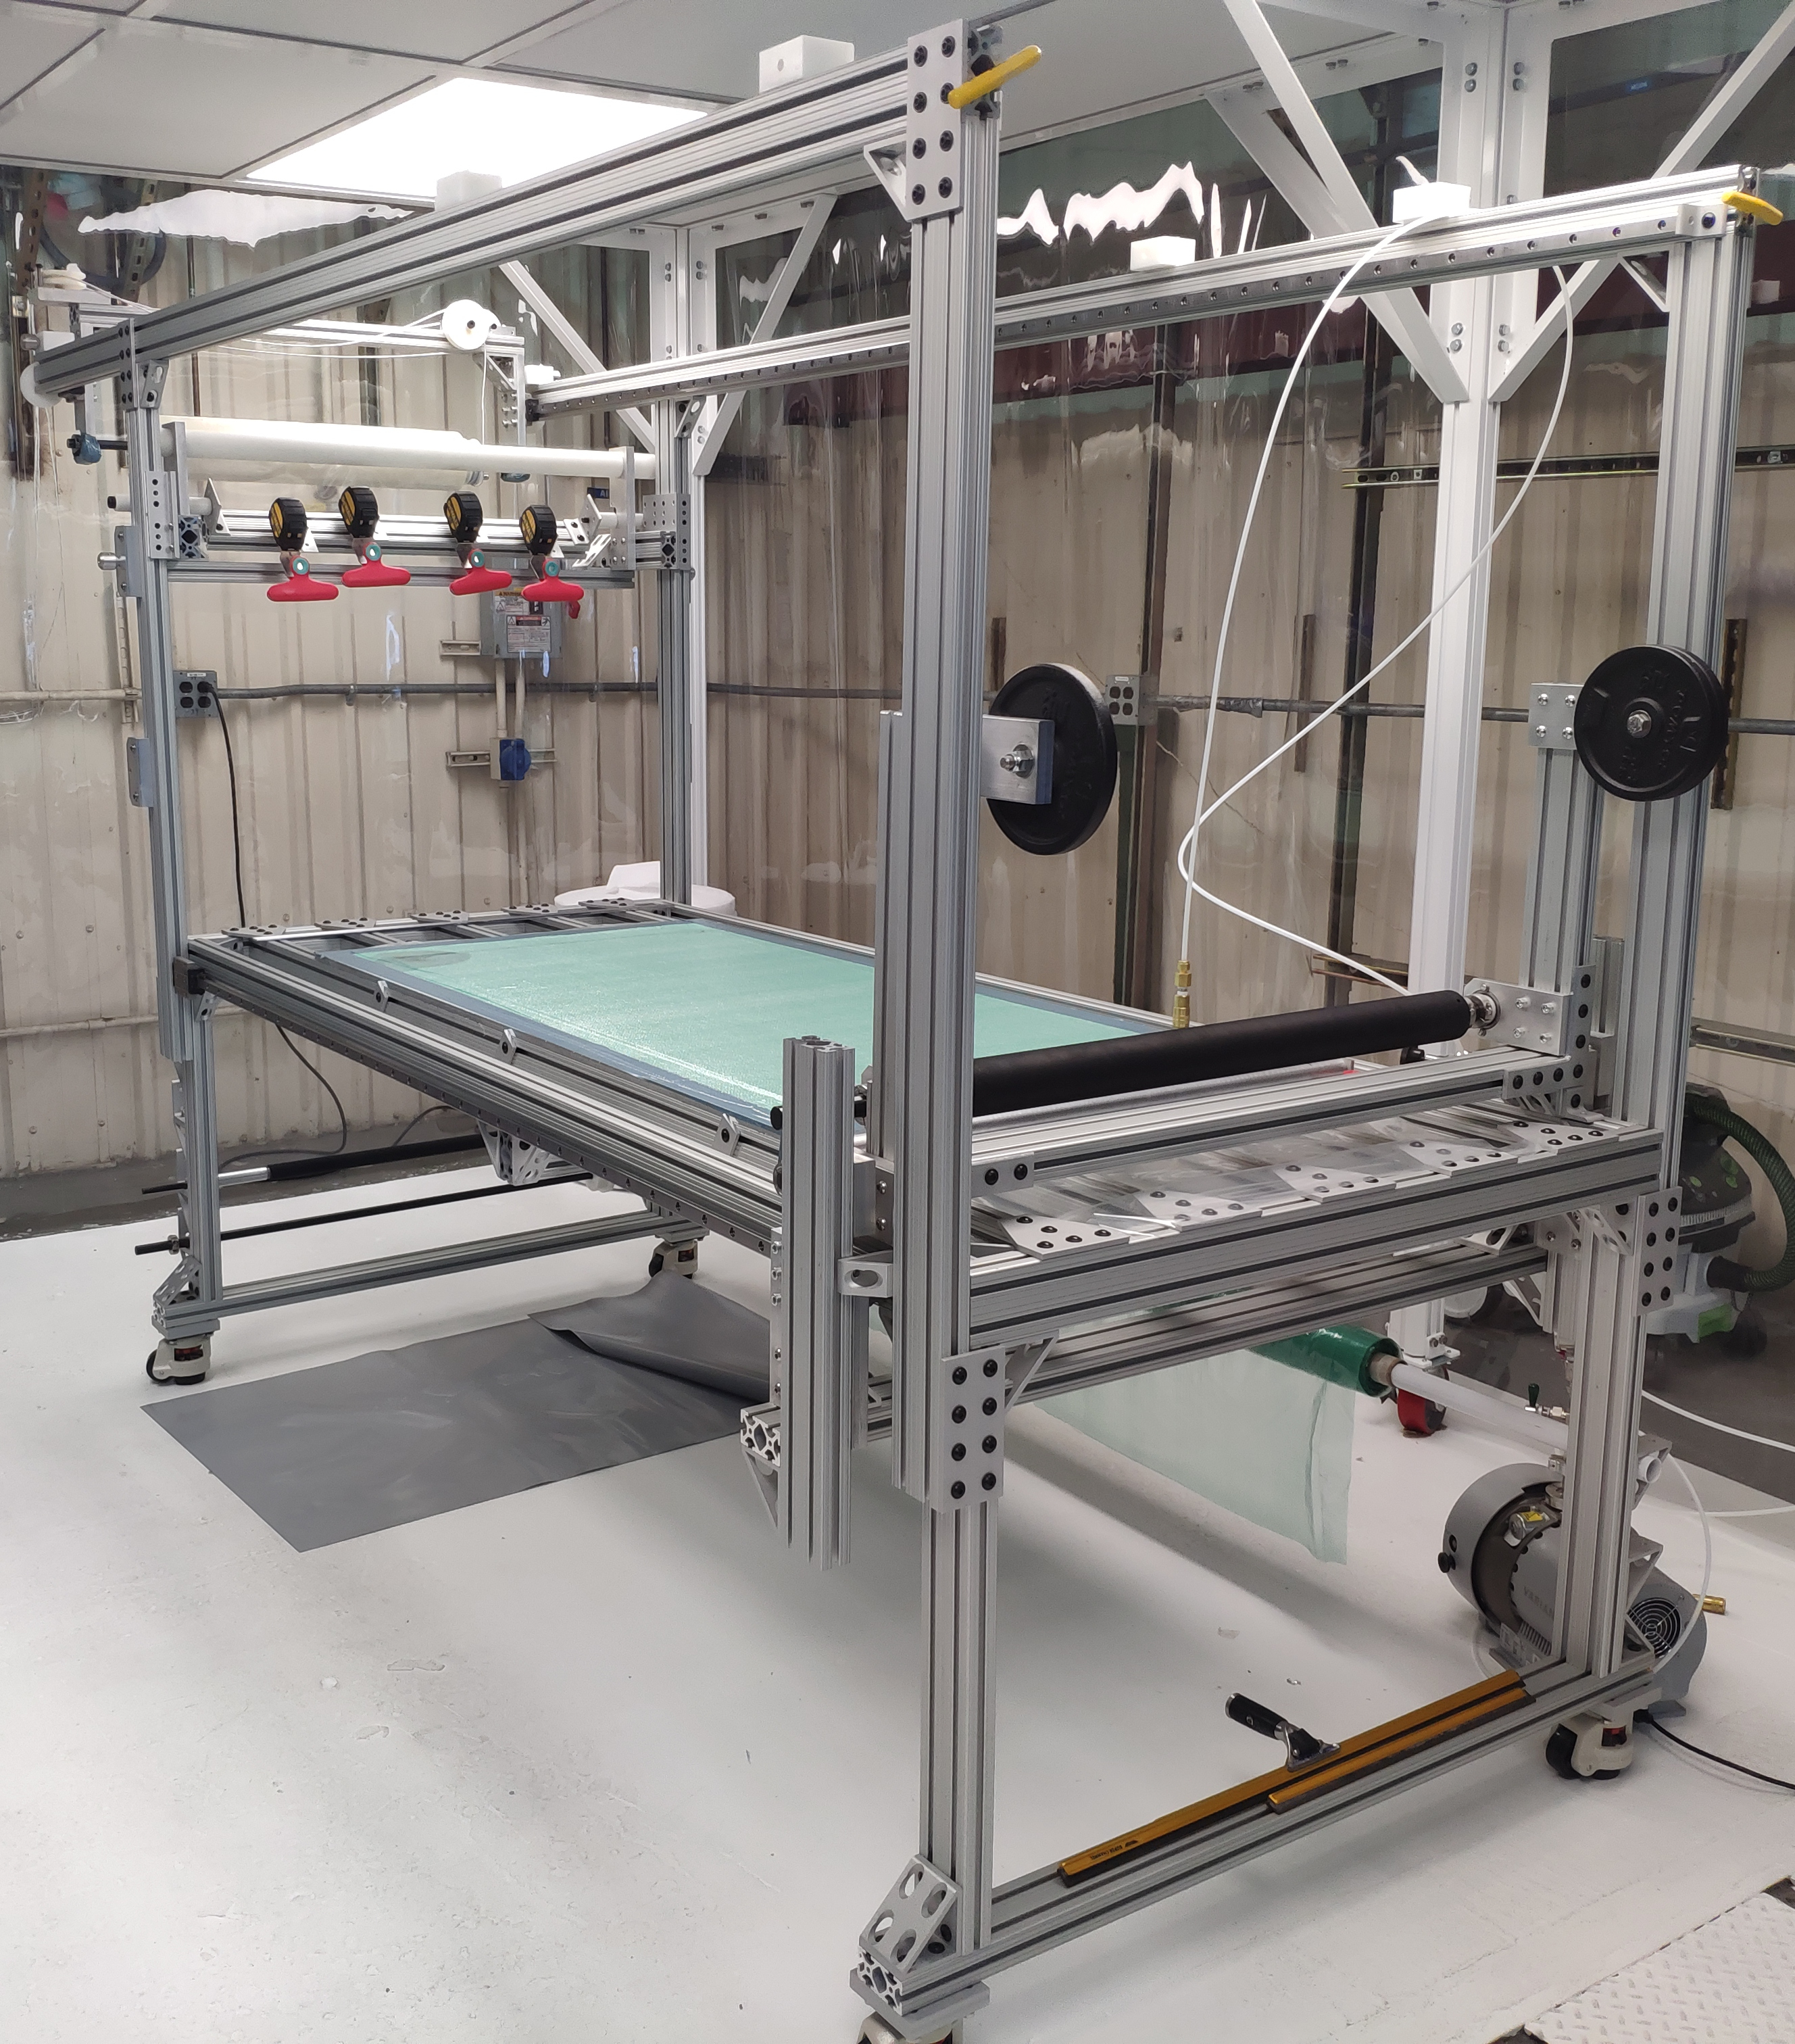
\includegraphics[width=\linewidth]{laminator.jpg}
		(a)
	\end{center}
\end{subfigure}
\qquad
\begin{subfigure}[c]{0.5425\linewidth}
	\begin{center}
		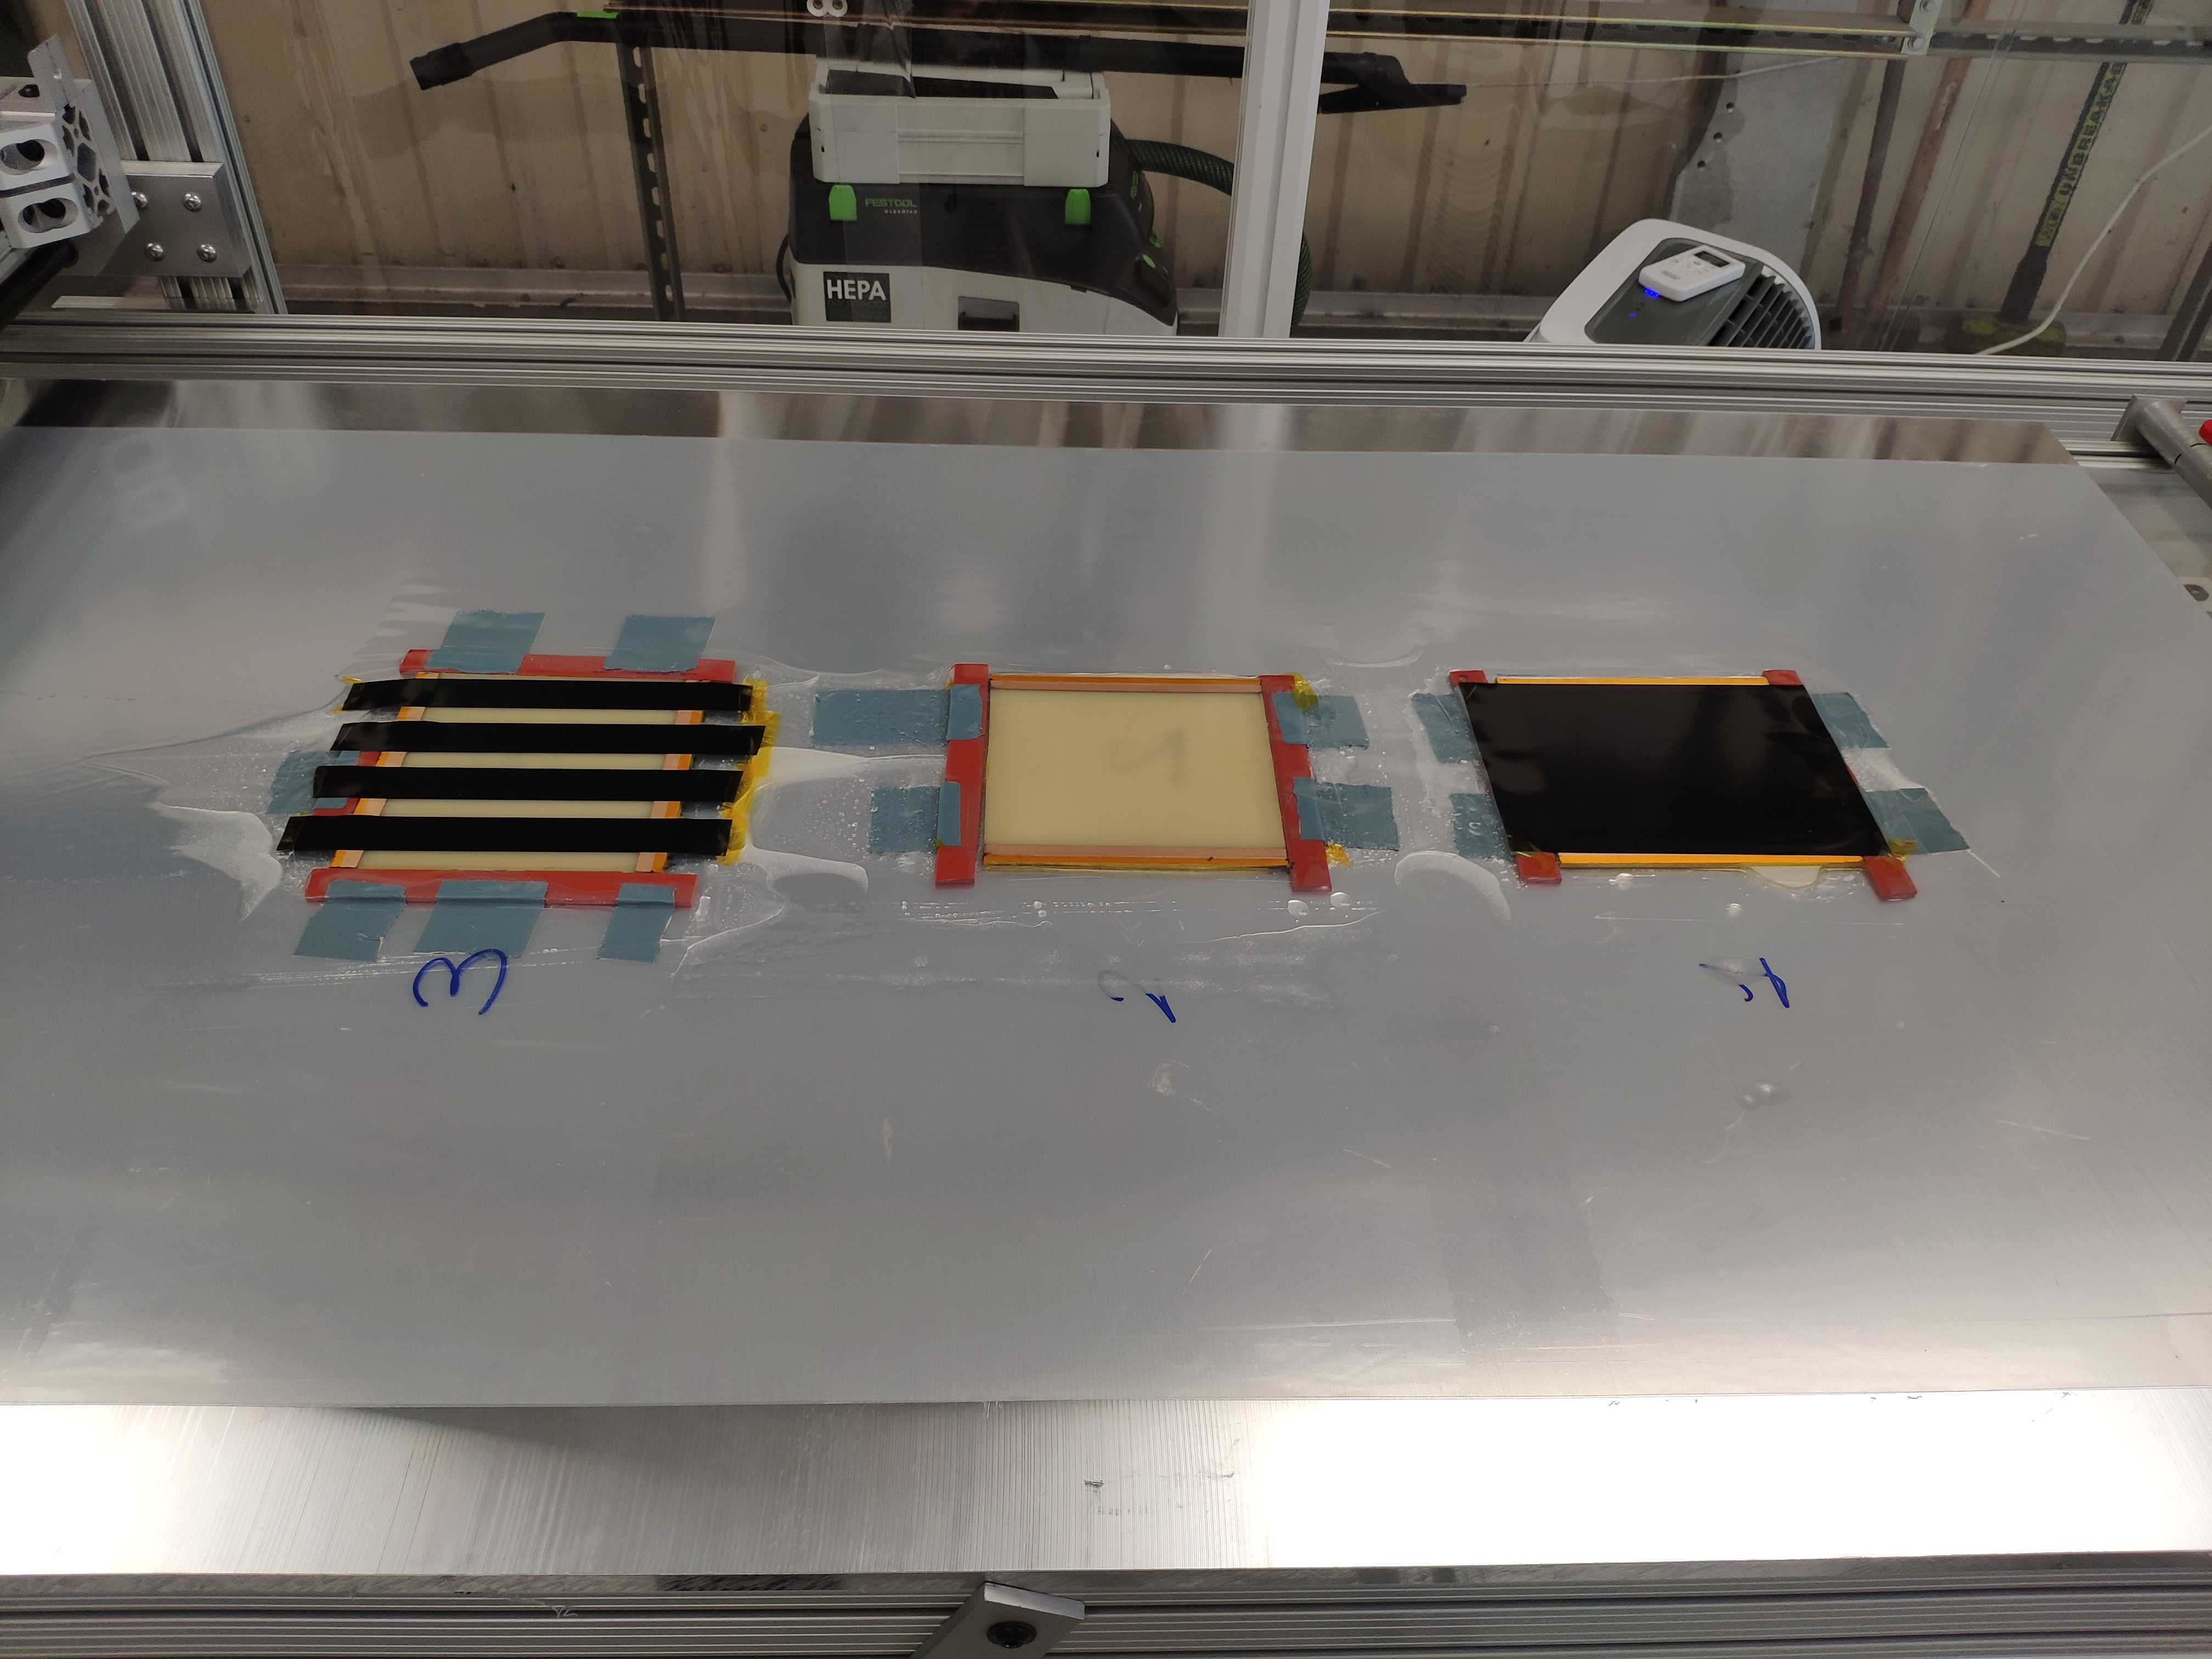
\includegraphics[width=\linewidth]{laminations.jpg}
		(b)
	\end{center}
\end{subfigure}
\caption{(a) Lamination device used to adhere Kapton onto FR4 panels. (b) Small $15\times15$\,cm$^2$ test panel laminations; left to right: zebra, alternate material (not discussed), full.}
\label{fig:field_shell_laminations}
\end{figure}

\todo{Francois: Replace with SLAC single cube panels. Consider adding picture of panel being laminated }



\subsection{Samples}
\label{sec:alt_samples}
For both the zebra and ladder designs, several parameters can be adjusted. In the zebra design, the {\DR} strip width, $w_s$, and the number of strips, $n_s$, can be adjusted to yield a bulk resistance of $R_z=\frac{L}{n_sw}R_S$ with $L$, the distance between the cathode and the anode and $R_S$ the sheet resistance of {\DR}. In this study, two sets of parameters were tested: $w=12.7\,$mm and $n_s=6$ (Z1) and $w=19.5$\,mm, $n_s=4$ (Z2).

In the ladder design, two additional free parameters can be set, the width of the gap between successive ladder steps, $w_g$, and the number of gaps, $n_g$. If the contact resistance between the {\DR} and the copper strips is negligible, the bulk resistance of the ladder is $R_l=\frac{n_gw_g}{n_sw_s}R_S$\RI{this usually doesnt look good, so either try to use \sfrac{1}{2} or make an equation out of it}. In this study, a single panel with $w_s=w_g=12.7\,$mm (L1), $n_s=3$ and $n_g=7$ was used. Note that, for a given $L$, the perceived electric field between ladder steps is greater than in the baseline design, as the width of the steps is finite and the total distance is thus $n_gw_g<L$. Figure~\ref{fig:shell_designs_picture} shows the three aforementioned test panels along with a laminated baseline design panel.

\begin{figure}[htbp]
\centering
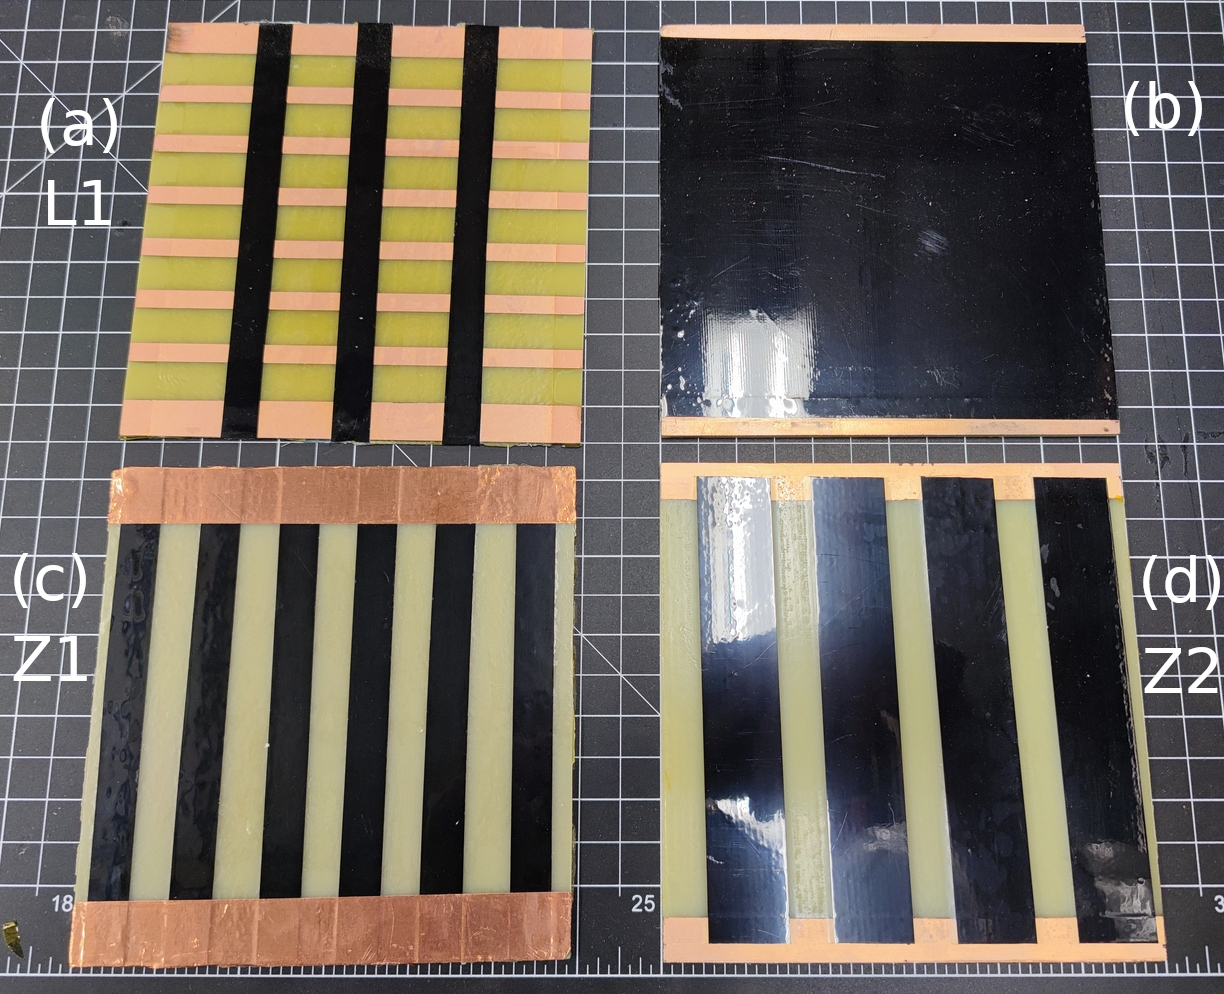
\includegraphics[width=.75\linewidth]{field_shell_designs.jpg}
\caption{Samples under study in the field shell design comparison. (a) ladder design, (b) baseline design, (c) zebra design Z1 and (d) zebra design Z2.}
\label{fig:shell_designs_picture}
\end{figure}

\subsection{Measurement plan}


\subsection{Experimental Operation}
\label{sec:ExpOp}

\RI{for run 0, we did voltage scan, for run 1 we did drift measurements}

The system was tested  in a series of commissioning runs that included a full cycle of operation: $(a)$ activating the purifier;  $(b)$ filling the system with LAr; $(c)$ collecting data in stable conditions; $(d)$ evacuation of argon. The SC readings for a typical operation of steps $(b) - (d)$ are shown in Figure~\ref{fig:stab}.

To activate the purifier the sieves within are regenerated i.e., water and $O_2$ molecules are evacuated from the sieves. The process of regenerating both sieves is based on Temperature Swing Adsorption (TSA)~\cite{LeVan1989}. For the molecular sieves, the entire nipple is externally heated to ~200\,C$^{\circ}$ using heating tapes and kept at that temperature for 24\,hours, this insures the inner volume is entirely heated, after 24\,hours $N_2$ is flushed through the system and is purged through a designated valve (V5 in Figure~\ref{fig:pnid}). At first water comes out and after a short while only humid $N_2$ does, the humidity level is monitored and when drops below the sensitivity of the meter (few percent) the heating is turned off, valves are closed and the system cools down for about 24\,hours. For the Copper sieve the same procedure is used except argon balanced hydrogen is used (2\% hydrogen). The hydrogen molecules attach to the $O_2$ molecules in the copper sieves to form water, we continue this until the humidity drops to a few percents and let the system cool back down. Additional micrometer filters are mounted between the purifier and the main dewar to prevent debris from the sieves to get into the main dewar.

After the purifier has been regenerated, the process of filling can start. We use certified ultra high pure LAr (six grade) filling dewar with a pressure of 220\,bar. In order to cool down the purifer we position an open mouth dewar around it, and fill it with LAr. Once Purifier is cold the filling of the main dewar can start. The flow supplied to the system is controlled manually by the valve on the filling dewar. The pressure on the purifier is kept at (2-2.5)\,bar. The LAr entering the main dewar evaporates immediately and evacuated through the BPR or PRV. The evaporated LAr also evacuates any gas that was inside the main dewar prior filling. Once the dewar is cold enough LAr starts to accumulate.

When the temperature on the TS drops below 0\,C$^\circ$ the TS is filled gradually with $N_2$. This process continues until the TS is filled with 60 standard liters (at room temperature and pressure) of $N_2$, once steady state is achieved this amount results in the TS bottom part being full. 

The entire filling takes $\sim2.5$\,hours until the liquid level reaches the desired level (one inch above the roll sock). At that point the system is left for 24 hours to reach steady state and more LAr is needed it is added then. Throughout the filling we apply a voltage of 1\,kV to get temperature dependency measurement.

At the end of a run, to speed up the evacuation of LAr, the heater attached to the copper brick at the bottom of the dewar is operated and supplies 150\,W of heating to evaporate the LAr, the evaporated LAr is exhausted through the BPR and PRV until the dewar is empty. The HV is set to 5\,kV to get another temperature dependency measurement. 



\subsection{Stability}
\label{sec:stab}
\todo {does this need it's own section, suggest combine with above.}

\todo{Francois: remake the plot, useful to see how long we ran (better than hours -> days). remake style}


\begin{figure}[htb]
	\centerline{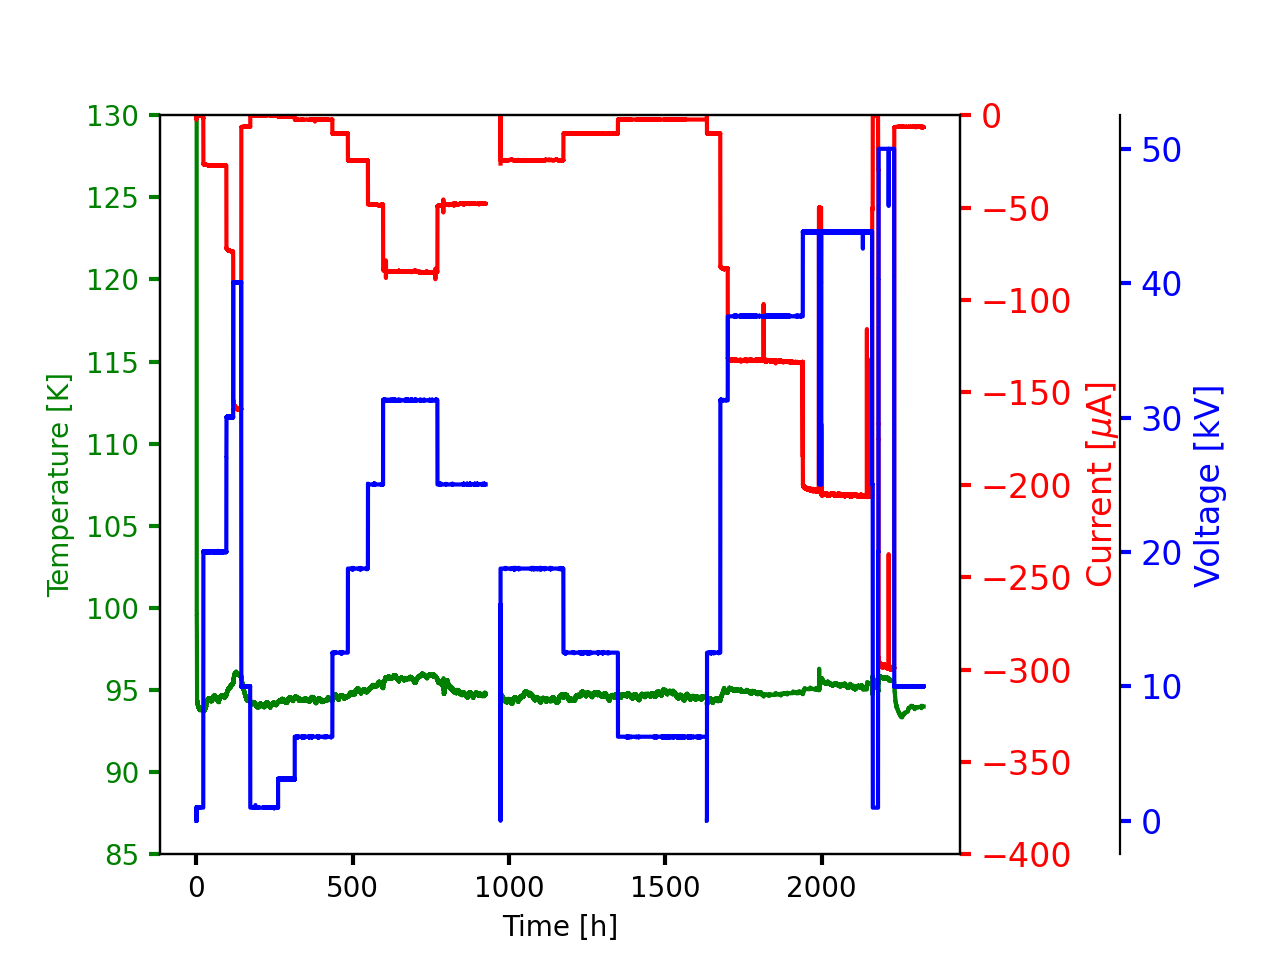
\includegraphics[width=\linewidth]{longrun.png}}
	
	\caption{Our recorded run, with the DR8 temperature, chosen voltage, and recorded current. \RI{Can we make solid rectangles over down times.. also this caption needs much more info, finally can you try to produce this plot a bit less symmetric (maybe make x=1.5y in length)} }
	\label{fig:stab}
\end{figure}
In this section, we will discuss the long, mostly continuous operation of our system across a range of voltages. The goal of this run is two-fold. First, we wish to explore the behavior of Kapton DR8 at a wide range of electric field intensities and verify its high resistance for use in DUNE ND and other TPCs. Second, we want to verify the behaviour and stability of Kapton DR8 over a long period of time, as, for the intended use case, this material will need to operate at a target voltage uninterrupted in liquid argon for years without replacement. Finally, we want to characterize its breakdown electric field regime and possible rate of breakdown. We do this so we can be confident that even at electric fields much larger than 500V/cm, the material will remain stable. Presented in Figure~\ref{fig:stab} is the record of our long run. During this approximately 20 week run starting from 11/12/2020, we were interrupted FILL IN LATER times: twice due to a software bug in our DAQ, once due to a lab power outage, and finally once due to evaporation of argon below the pill months into the run. However, none of these stoppages were the result of any electrical failure on the part of the system.

We begin our scan with a couple days each at 20kV, 30kV, and 40kV, followed by a return to DUNE ND design electric field of 500 V/cm, or 6.125kV. At this stage we ramp up in voltage in multiples of 6.125kV up to 31.25kV, again taking at most a couple days at each step, before stepping down again to 6.125kV with the same steps, but for approximately a week at each run.
At the end of this ramp down, we experience a lab power outage, explaining the second gap in Figure~\ref{fig:stab}. We will compare the resistivity before and after the ramp in the following section, in order to ascertain the existence of any resistive decay from this process. With this complete we continue the second ramp up from 31.25kV to 50 kV with the same steps, analyzing the behavior and resistive decay of the sample at these much higher voltages.



\section{Results}
\label{sec:res}
% @Zach: Some sentences here are needed before diving in just to introduce this section, for example we present results from all aperatai, where he specific apparatus used will be mentioned at the beginning of the relevant sections. For LAIR2 we use the data from our run XXX which is described in Sec~XXX, for the rest we use dedicated specific measurements.   
\subsection{Temperature Dependence}
\label{sec:TNEFit}
% @zach I think I would start with something that is saying fitrst how do we measure the T dep. say something like, In ordr to quantify the depandance of the resistance with T, the data from the cooling down of the system is used. This data spans over the temperature range of XXXX
The results in this section are obtained from the LAIR2 apparatus (see section~\ref{sec:expsetup}). The measured current exhibits modest temperature dependence which is well modelled by a general hopping transport model (see eq.~\ref{eq:Tdep}), following~\cite{electronicPhotonicMaterials} for the low temperature regime, we make the assumption that $\beta=0.5$. Using the data obtained when the system is cooling down, spanning the temperature range of (278--90)\,K, we get a temperature dependence that follows

\todo{Francois talk to Dan and decide on best way to remake this plot. Fig 10- nice to show 1/sqrt(T) see linear dependance but the problem is that the reader can’t see it to temperature-- find resistance of operation.
}
% 

\begin{equation}
\label{Rmeas}
R_{s}^{meas}(T)=R_s\exp\bigg(\sqrt{\frac{T_0}{T}}\bigg),
\end{equation}
where $R_{s}^{meas}(T)\equiv V/I$ is the measured sheet resistance and $R_{s}$ and $T_0$ are temperature-independent fit coefficients, with $R_s =0.021 G\Omega/\Box$ and $T_0 = 3152.38~K$, see Figure~\ref{fig:cooldown}. 
% @Zach Can you say something on how you got these coefficients?

\begin{figure}
\centering
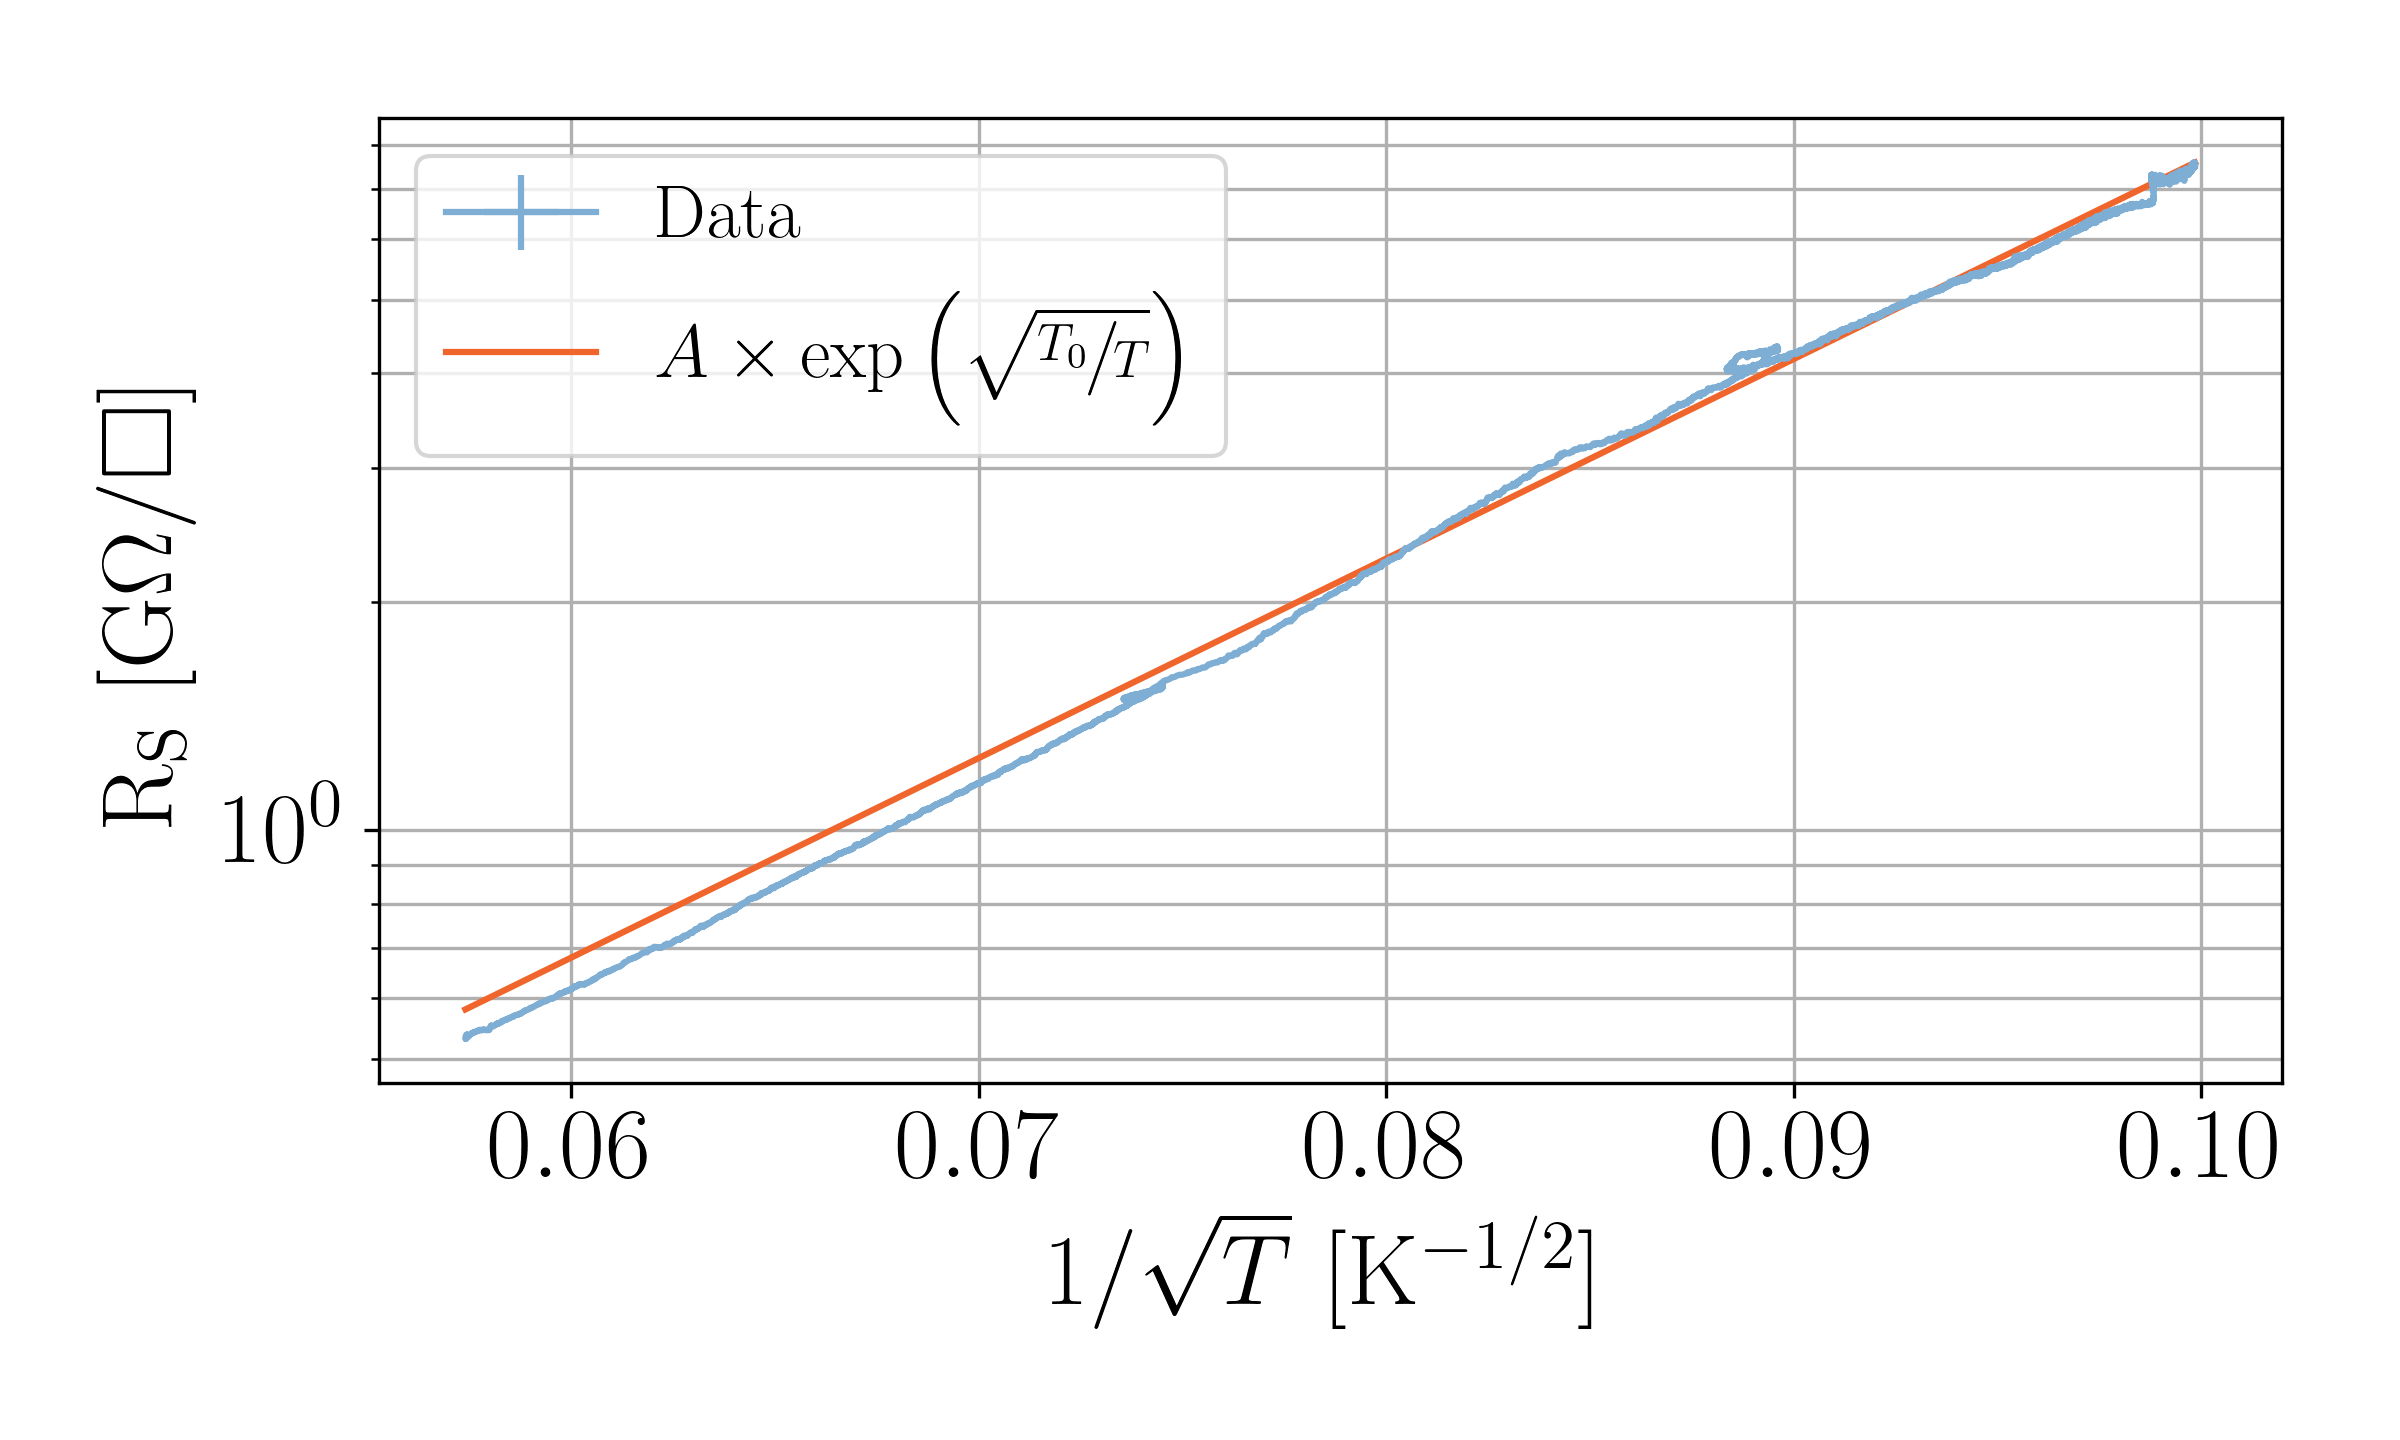
\includegraphics[width=0.95\textwidth]{temp_sheetRes_dr8_cooldown.png}
\caption{The observed resistivity of a sample of DR8 as a function of temperature, taken at a field of 80 V/cm. We also show excellent fit with the model from Eq. \ref{Rmeas}. \RI{Zach is this an old plot, not from the time period I gave you ?}}
\label{fig:cooldown}
\end{figure}
% @Zach, this is unclear, maybe you should say something, like: For the rest of the analysis we integrate-out the temperature depandance by normalizing to a temperature of 95K which is close to the working temperature (question: is this true isnt it better to choose 92) (note that this temeprature choice is arbitrary and is chosen to this value for connivance ) 
In order to extract the dependence of the resistance on the applied electric field, the temperature dependence needs to be taken into account. We normalize the rest of the measurements to a temperature of (95\,K) using 
\begin{equation}
R_{s}^{meas}(95)=R_{s}^{meas}(T')\exp\bigg(-\sqrt{\frac{T_0}{T'}}+\sqrt{\frac{T_0}{95}}\bigg).
\end{equation}
where $R_s^{meas}(95)$ is the resistance at 95\,K $T'$ is the temperature measured, and $R_{s}^{meas}(T')$ is the measured resistance at the measured temperature. 

\subsubsection{Temperature Measurement Uncertainties}
\todo{zach start with there are several sources of unc for this measurements, give a quantification of them or a sentence we conclude they are negligible for the purpose of T dep. also try not to wirte fraction inline use / instead of sfrac. side note, Im not sure I would even discuss this entire thing if the conclusion is that it is negligible. I doubt someone will imagine that the T measurement is not done adequately and that we need to explain. If referee asks we can give hime this calculation.}  
One source of uncertainty for us is the placement of our temperature sensor. While in the vicinity of the sample and roughly at the same vertical level, we place the sensor a couple inches away in order to minimize possible arcing when ramping up all the way to higher voltages. This results in a slight delay of temperature propagation from the sample, loss of contact heat-transfer, as well as a reduction in correlation from localized temperature changes driven by the heat of the sample itself. In order to characterize the possible extent of this temperature difference, we model our system as a vertical sheet in liquid argon, with one temperature sensor on the sample, and one infinitely far away, and we calculate the steady state difference between the two with heat transfer dynamics governing the system. In other words, we note that, for a sample surrounded by a steady temperature, the heat lost from contact with the liquid argon has to equal the resistive heat generated, or that $\frac{dQ}{dt}=hA(T_{\infty}-T_{sample})+IV=0$, where $h$ is the heat transfer coefficient which needs to be calculated, $A$ is the surface area of the board, and the final term is the power generated from the sample itself.

Following the equations in~\cite{CHURCHILL19751323} for free convection near a vertical wall, where we have adjusted the gravitational constant to reflect the 30 degree incline of our sample as well as ignored the FR4 board on one side of the sample, we insert the characteristic length of our material, 6 inches, as well as approximate thermodynamic and material properties of liquid argon around our pressure. We need a liquid argon density, $\rho=1.396\frac{g}{ml}$, a specific heat, $c_p=45\frac{J}{mole \cdot K}$, a viscosity, $\mu=270.7(10)^{-6}Pa s$, a thermal conductivity, $k=0.1256\frac{W}{m K}$, and a coefficient of thermal expansion $\beta=4.55(10)^{ -3}/K$~\cite{GLADUN1971205}\cite{STREETT197459}\cite{lbnl}. As $h$ is a function of $\Delta T$ as well, we have $\frac{dQ}{dt}(\Delta T)=0$, and thus we can find $\Delta T$ by root-finding. We find that the difference in the two sensors at 12.5kV would be around 0.03K, while the difference in the two sensors at 50kV would be around 1.3K. From these rough estimates, we can conclude that across all measured voltage regimes, the temperature is almost entirely driven by the liquid argon, and the temperature sensor in the vicinity should be an accurate measurement of the temperature of the material. On top of that, our model for the temperature correction includes a constant, $T_0$, which absorbs any overall scaling between the true temperature of the sample and the measured value.

In previous tests, we also noted that at electric fields of approximately 1000V/cm and higher, both a pure FR4 board and a FR4 board with epoxy coating conduct to a degree at room temperature. However, upon immersing these boards in liquid nitrogen, the conductance decreased to the point of immeasurability. We thus conclude that the conduction shown in this paper is a result of purely DR8 conduction modes.

%\RI{Zach Can you Add a temperature correction plot, also, can we give a goodness of fit for the temperature fitting?}


%%%%%%%%%%%%%%%%%%%%%%%    Begin Comment %%%%%%%%%%%%%%%%%%%%%

\begin{comment}

%Ran Itay Im here

As we discovered during and after the run, a noticeable measurement uncertainty characterizes our low-voltage results, which we believe to be from a combination of factors. For one, our system does not have an independent measurement of the voltage from the power supply, although the power supply itself does record a value. From analysis of the experiment after the fact, we also found a small coupling between our temperature sensors and the return line. Separating these two systems after the run resulted in a cleaner signal at low voltages.

This noise decreases markedly at higher voltage, which allows us to continue with the analysis. However, we are unable to definitively model the source and size of the measurement uncertainty, independently of data.


We also experienced infrequent and unphysical spikes in the recorded measured current which subtracted from both the fits and the presentation of the signal. In order to counter this, after computing $\ln(R_s)$, we assign a local standard deviation and mean at each point in time, corresponding to a minute's worth of points. Then, we subtract any point which is more than 5 local standard deviations away from the local mean as an unphysical artifact.

As a final note, the very beginning of each voltage interval, after having changed from one voltage to the next and thus from one stable local temperature to the next, exhibits transient temperature behavior, and thus in our fits, we ignore the first 2 hours of any voltage interval, although we still plot these points.



%We record the sheet resistances across a wide range of voltages and at various temperatures, and thus we require a convention for what "the sheet resistance" at a particular voltage means. To eliminate the temperature dependence from each curve in a consistent way, and to compare each sheet resistance curve in similar conditions, we employ the following temperature "normalization" for sheet resistance curves taken at different temperatures:
%\begin{equation}
%R_{s}^{meas}(T)=R_{s}^{meas}(T')\exp\bigg(-\sqrt{\frac{T_0}{T'}}+\sqrt{\frac{T_0}{T}}\bigg).
%\end{equation}
%In this paper we compare all curves at the choice of constant $T=95K$, so all plots of sheet resistance are plots of $R_{s}^{meas}(95~K)$. Thus this equation represents our corrections of sheet resistance variations due to temperature.
\end{comment}
%%%%%%%%%%%%%%%%%%%%%%%%%    End Comment %%%%%%%%%%%%%%%%%%%%%
\subsection{Electric Field Dependence}
\label{sec:efield_dep}
\begin{figure}
\begin{center}
	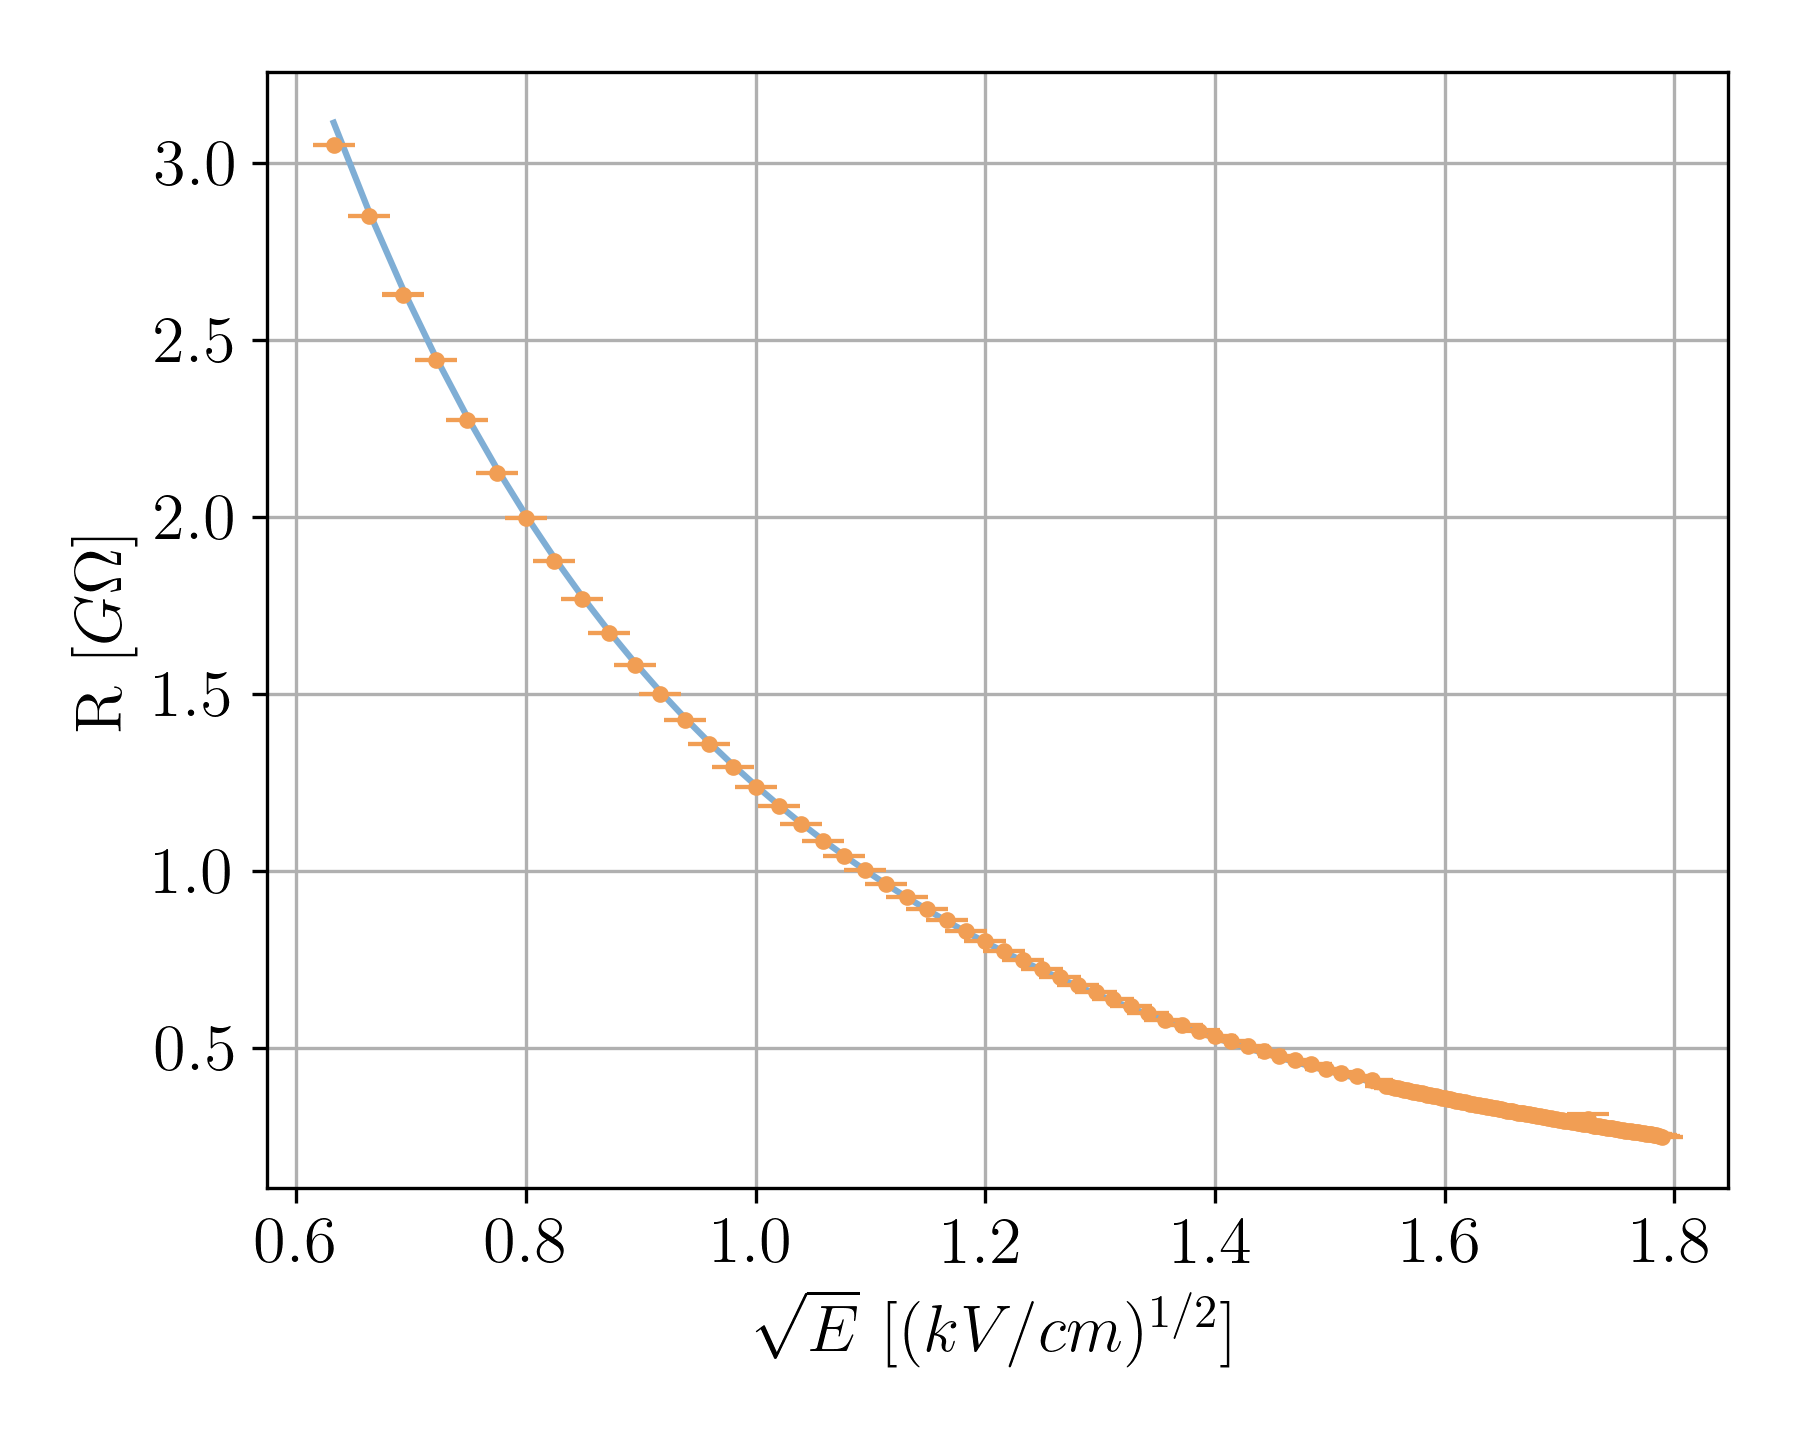
\includegraphics[width=.75\linewidth]{Efield.png}
	\caption{Resistance as a function of square root electric field, with fit to the Hopping model plus additional parameter.}
	\label{fig:resvsvol}
\end{center}
\end{figure}

\todo{FD: Fig 11, should be log scale for y axis; talk to Dan to remake it. Also, are there any lower field measurements?}

As discussed in section \ref{sec:disorder_Mattrial}, in the temperature and voltage regime of interest, The resistivity of DR8 depends exponentially on the  square root of the electric field. To validate this, we scan electric fields ranging from $416$V/cm to $3200$V/cm and measure the current through our sample. Specifically, starting from $400$V/cm we increment the electric field in steps of $40$V/cm up to $2.4$V/cm, with multiple hour long stops at $1.2$V/cm and $2.4$V/cm before continuing to $3200$V/cm with shorter increments.
Converting the measured current into resistivity with the voltage recorded from the power supply, we can compare with 
\begin{equation}
R_s \propto  e^{( E / E_0)^{-\frac{1}{2}}}.
\end{equation}

% @Zach Re-phrase, say in addition we bla bla , or we improve the fit bla bla, or to get something we add bla bla. sayign we almost od this is more of a street talk, than scientific writing.
We will almost do this, but instead, we will include an additional fit parameter to the functional form of the material's electric field dependency:
\begin{equation}
R=R_0 e^{( E / E_0)^{-\frac{1}{2}}+a_0 E}.
\end{equation}
We have added a term linear in electric field in the exponent corresponding to a higher order term in the expansion of $\ln(R_s)$ with corresponding fit parameter, $a_0$. Shown in Figure~\ref{fig:resvsvol} is the result of the voltage scan and the excellent agreement with the fitted function. 


\subsection{Transmission Line Measurement}
\label{sec:transLine}

Transmission Line Measurement (TLM) is a standard method for measuring the resistance associated with the contact between two materials.  In this method, a series of samples are constructed with varying distances between contacts, and the resulting resistance is measured.  The resistance of a given sample is modelled as the sum of the resistance of the two contact patches and the resistance of the material itself.  The contact resistance is then measured as half of the limit of the measured resistance as the distance between contacts approaches zero.

\begin{equation} \label{eq:TLM}
\begin{split} 
	R_{\mathrm{total}}(L) &= 2 R_{\mathrm{contact}} + R_{\mathrm{sample}}(L), \\
	R_{\mathrm{contact}}  &= \tfrac{1}{2} R_{\mathrm{total}}(L = 0),
\end{split}
\end{equation}
where $L$ is the distance between contacts, $R_{\mathrm{total}}(L)$ is the total resistance of a sample of linear size $L$, $R_\mathrm{contact}$ is the contact resistance, and $R_{\mathrm{sample}}(L)$ is the bulk resistance of a sample of linear size $L$.


For this measurement, we used a designated {\DR} sample that  was cut to length and cleaned with ethanol.  On one side a "stationary" contact was made with conductive copper tape\footnote{3M 1181}, square with the edges of the sample.  A second contact was made at various distances from the first.  Care was taken to arrange the contacts so that their edges were as parallel as possible, so that the direction of current flow is perpendicular to the edges of the copper contacts.  This was achieved to do a degree such that the difference in the measured inter-contact distance between the two sides of the sample is $\sim 0.2\,$\,mm.  The recorded length is taken to be the average distance between the two copper stripes (edge to edge ), the deviation from the average value is considered as an uncertainty to the measurement.

% (1.292, 1.869, 2.544, 3.108, and 3.755\,cm)
We measure the current in the sample, applying voltages in the range of (0-5)\,kV. We repeat this measurement for five different distances (\sfrac{1}{2}", \sfrac{3}{4}", 1", 1 \sfrac{1}{4}", and 1 \sfrac{1}{2}") and in a bath of L\ch{N2} in the cryostat described in Figure~\ref{fig:msu_styro_setup}. The results of these measurements are shown in Figure~\ref{fig:TLM_length_I_and_R}. The resulting resistance associated with the contact interfaces, is shown in Figure~\ref{fig:TLM_length_contactRes}.  The measured contact resistance at 500\,V/cm, a field typical for the operation of a DUNE-ND, is $107.4\pm$ 54.6 M$\Omega$

\begin{figure}[htb]
\centering
\begin{subfigure}[c]{0.32\textheight}
	\begin{center}
		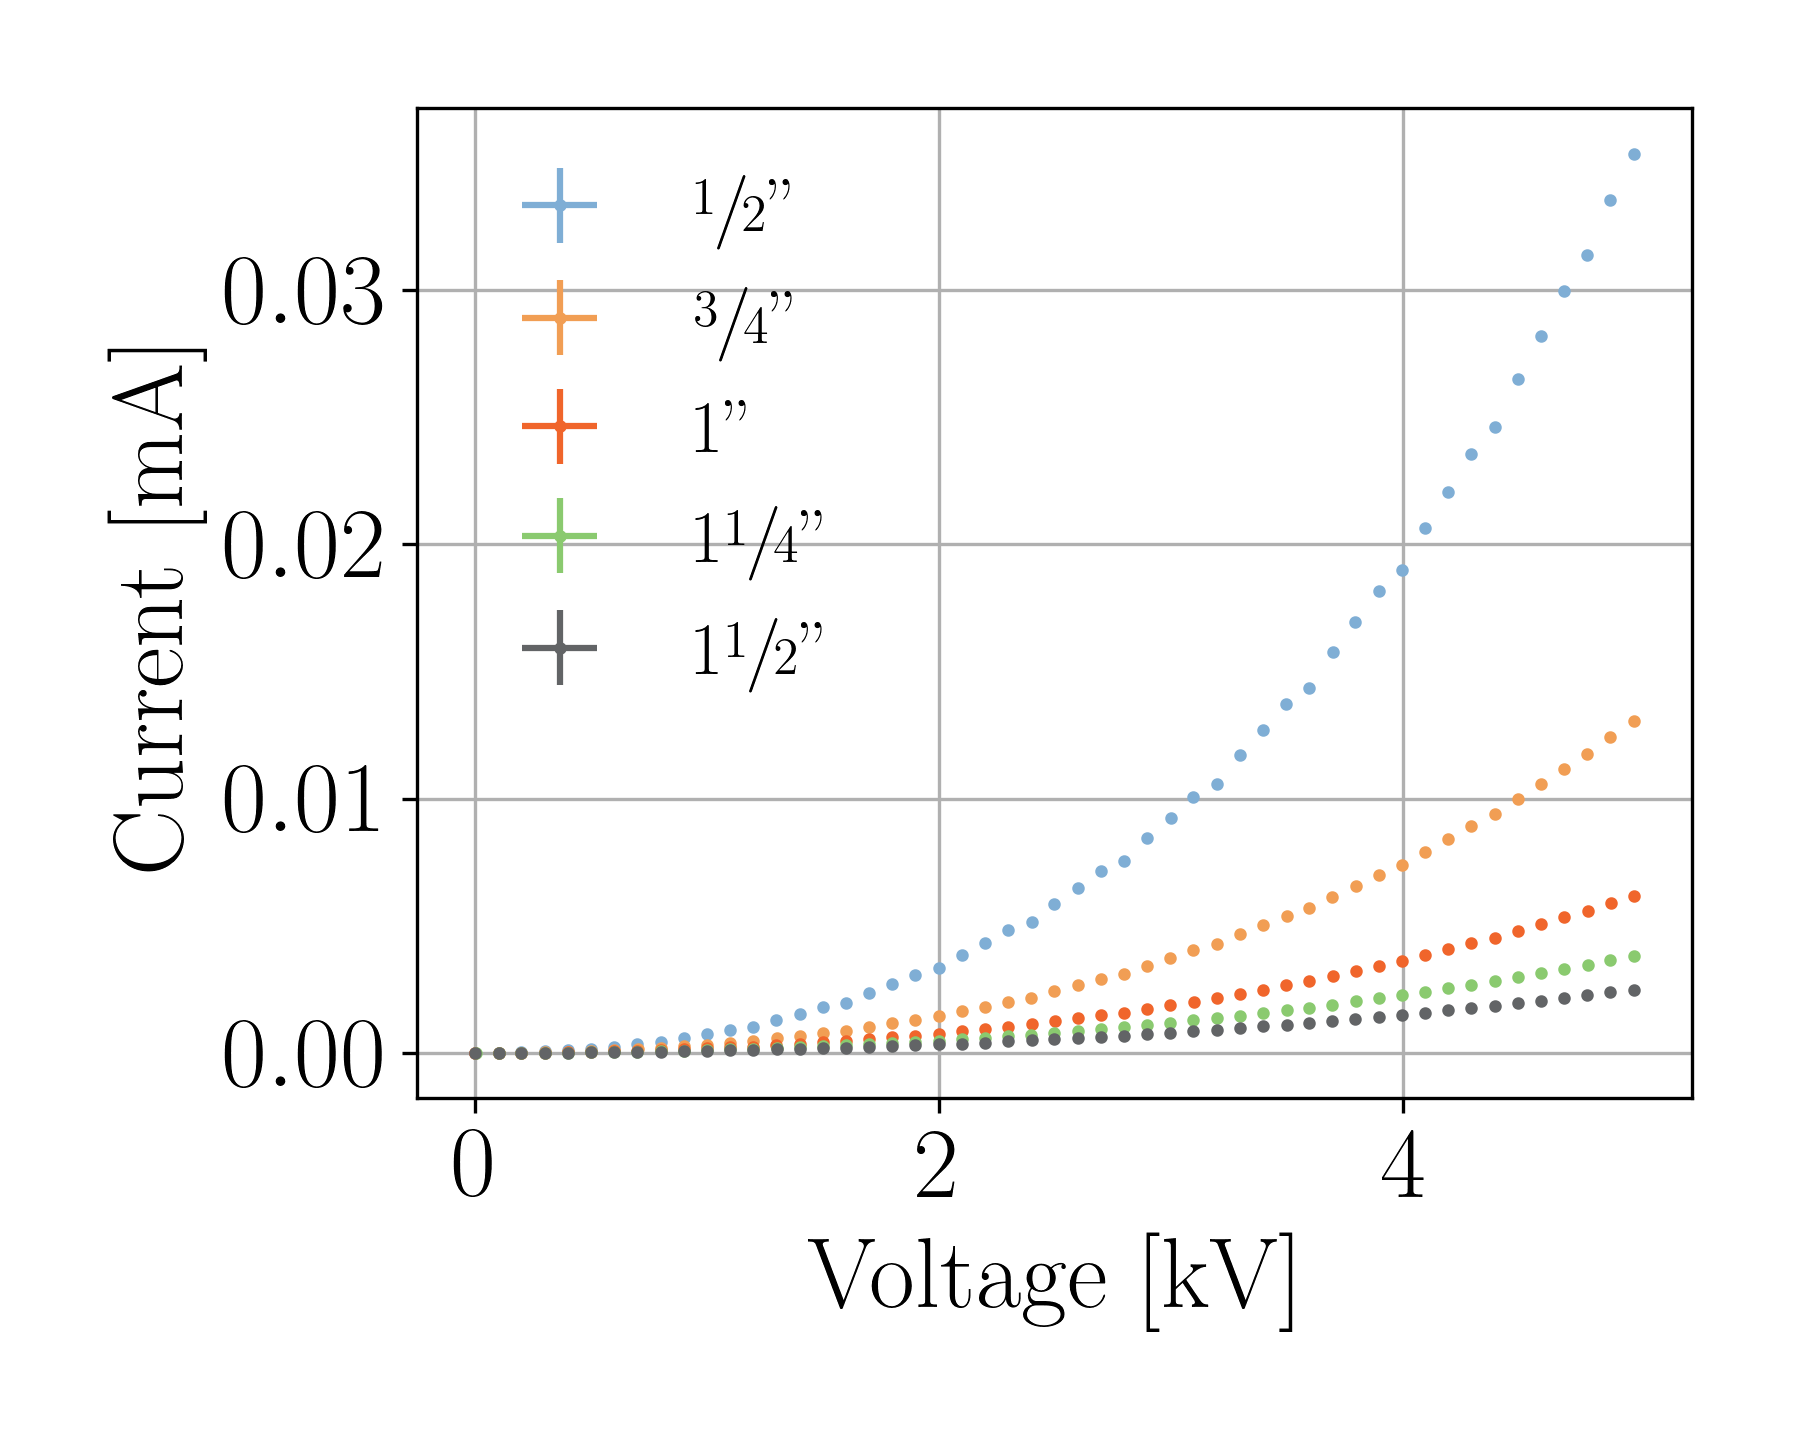
\includegraphics[width=\textwidth]{TLM_length_current.png}
		
		\vspace*{-\baselineskip} \hspace{1em} (a)
	\end{center}
\end{subfigure}
\begin{subfigure}[c]{0.32\textheight}
	\begin{center}
		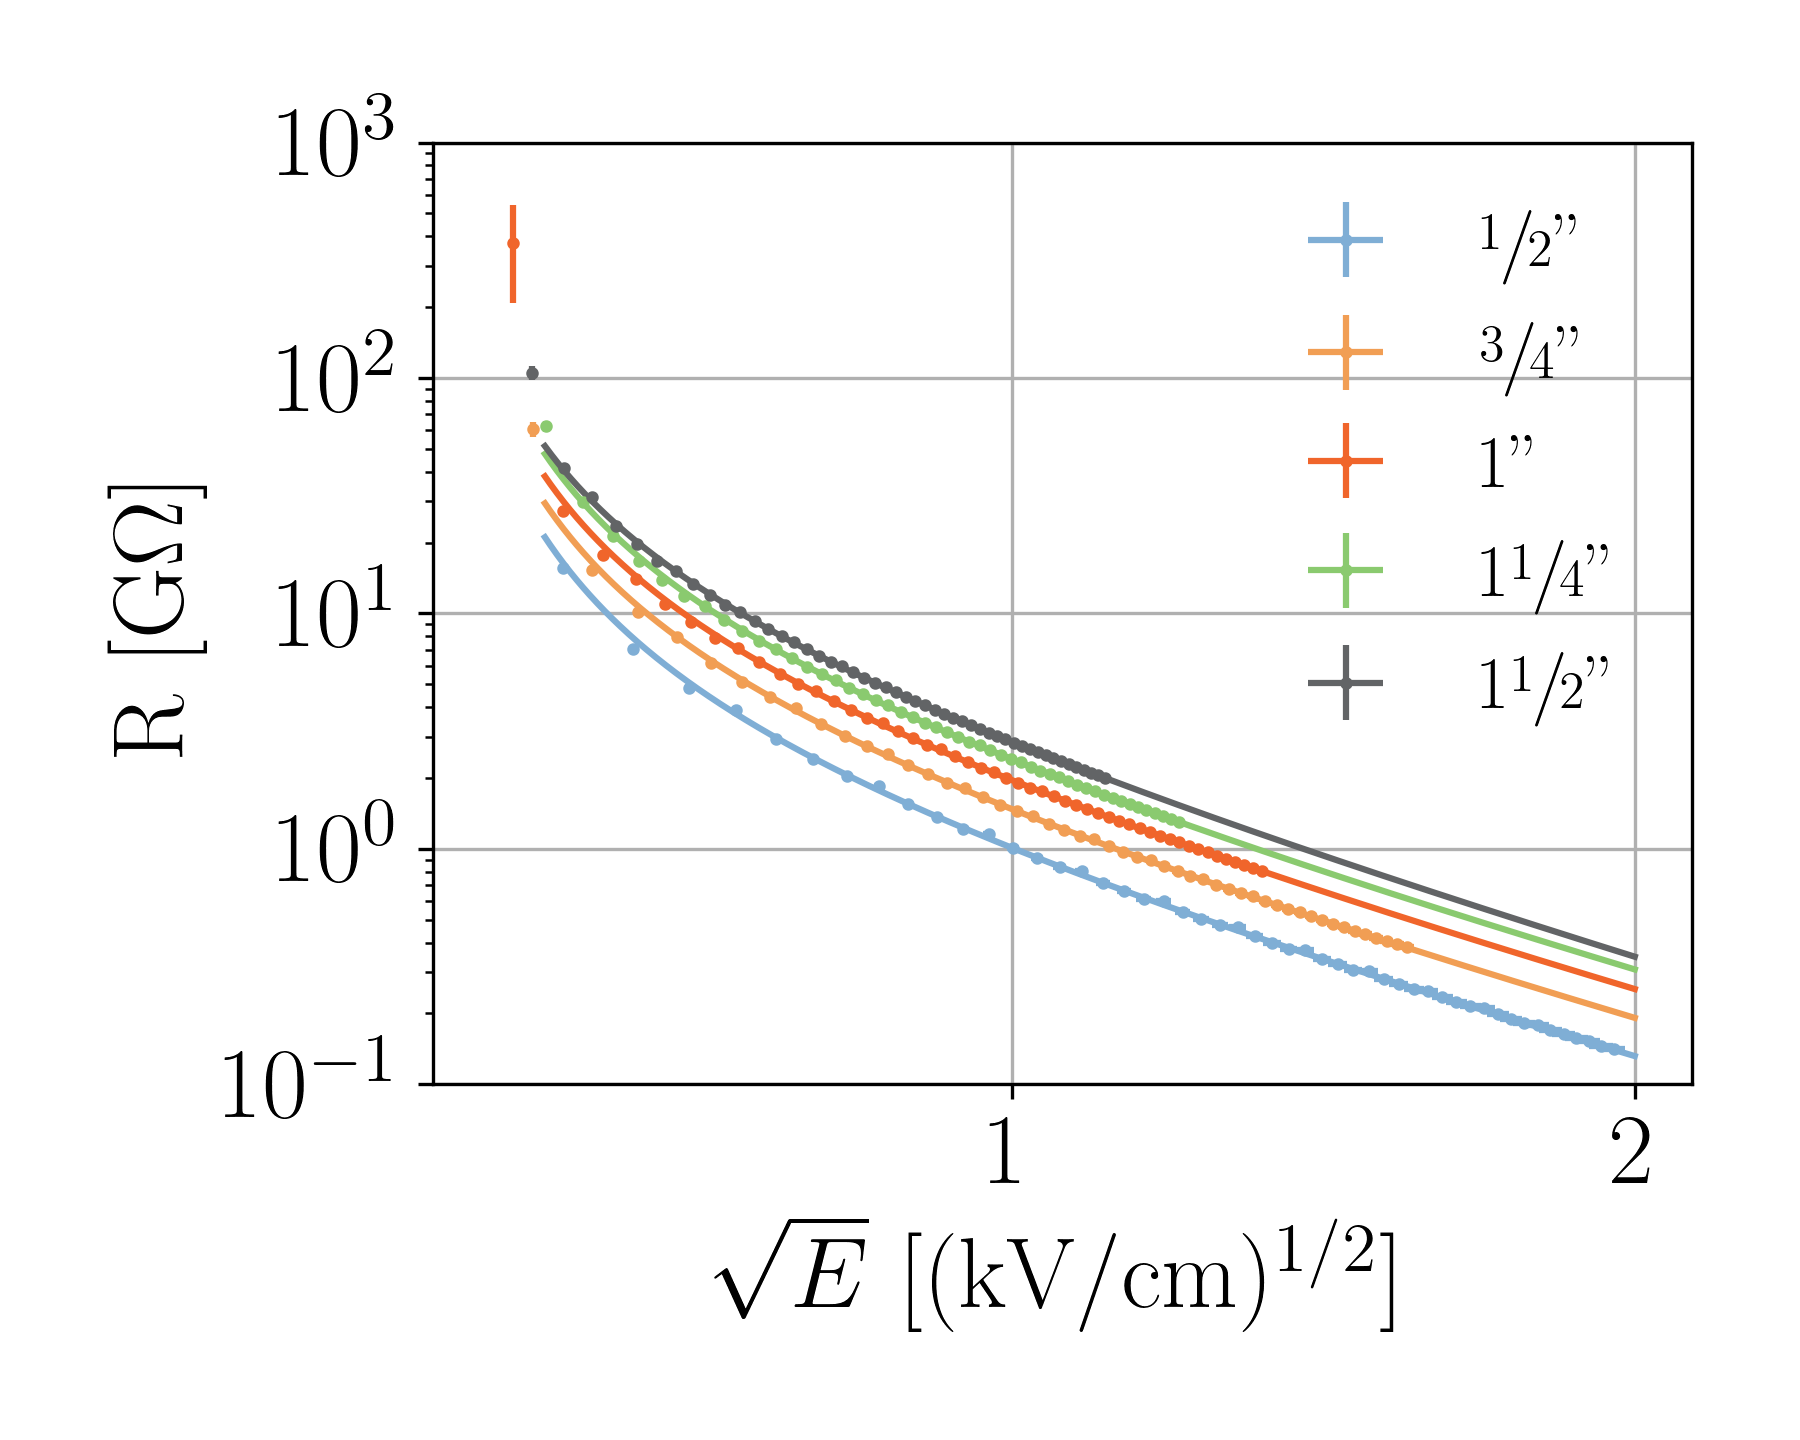
\includegraphics[width=\textwidth]{TLM_length_resistance.png}
		
		\vspace*{-\baselineskip} \hspace{2em} (b)
	\end{center}
\end{subfigure}
\caption{(a) The current measured as a function of voltage from each of the five samples considered. (b) The corresponding resistance as a function of the square root of the applied electric field values calculated from those measurements.  Note that the plotted model fits are essentially parallel, differing only by a multiplicative factor.} 
\label{fig:TLM_length_I_and_R}
\end{figure}

\todo{Increase size of this figure after clean up}


\begin{figure}[htb]
\centering
\begin{subfigure}[c]{0.32\textheight}
	\begin{center}
		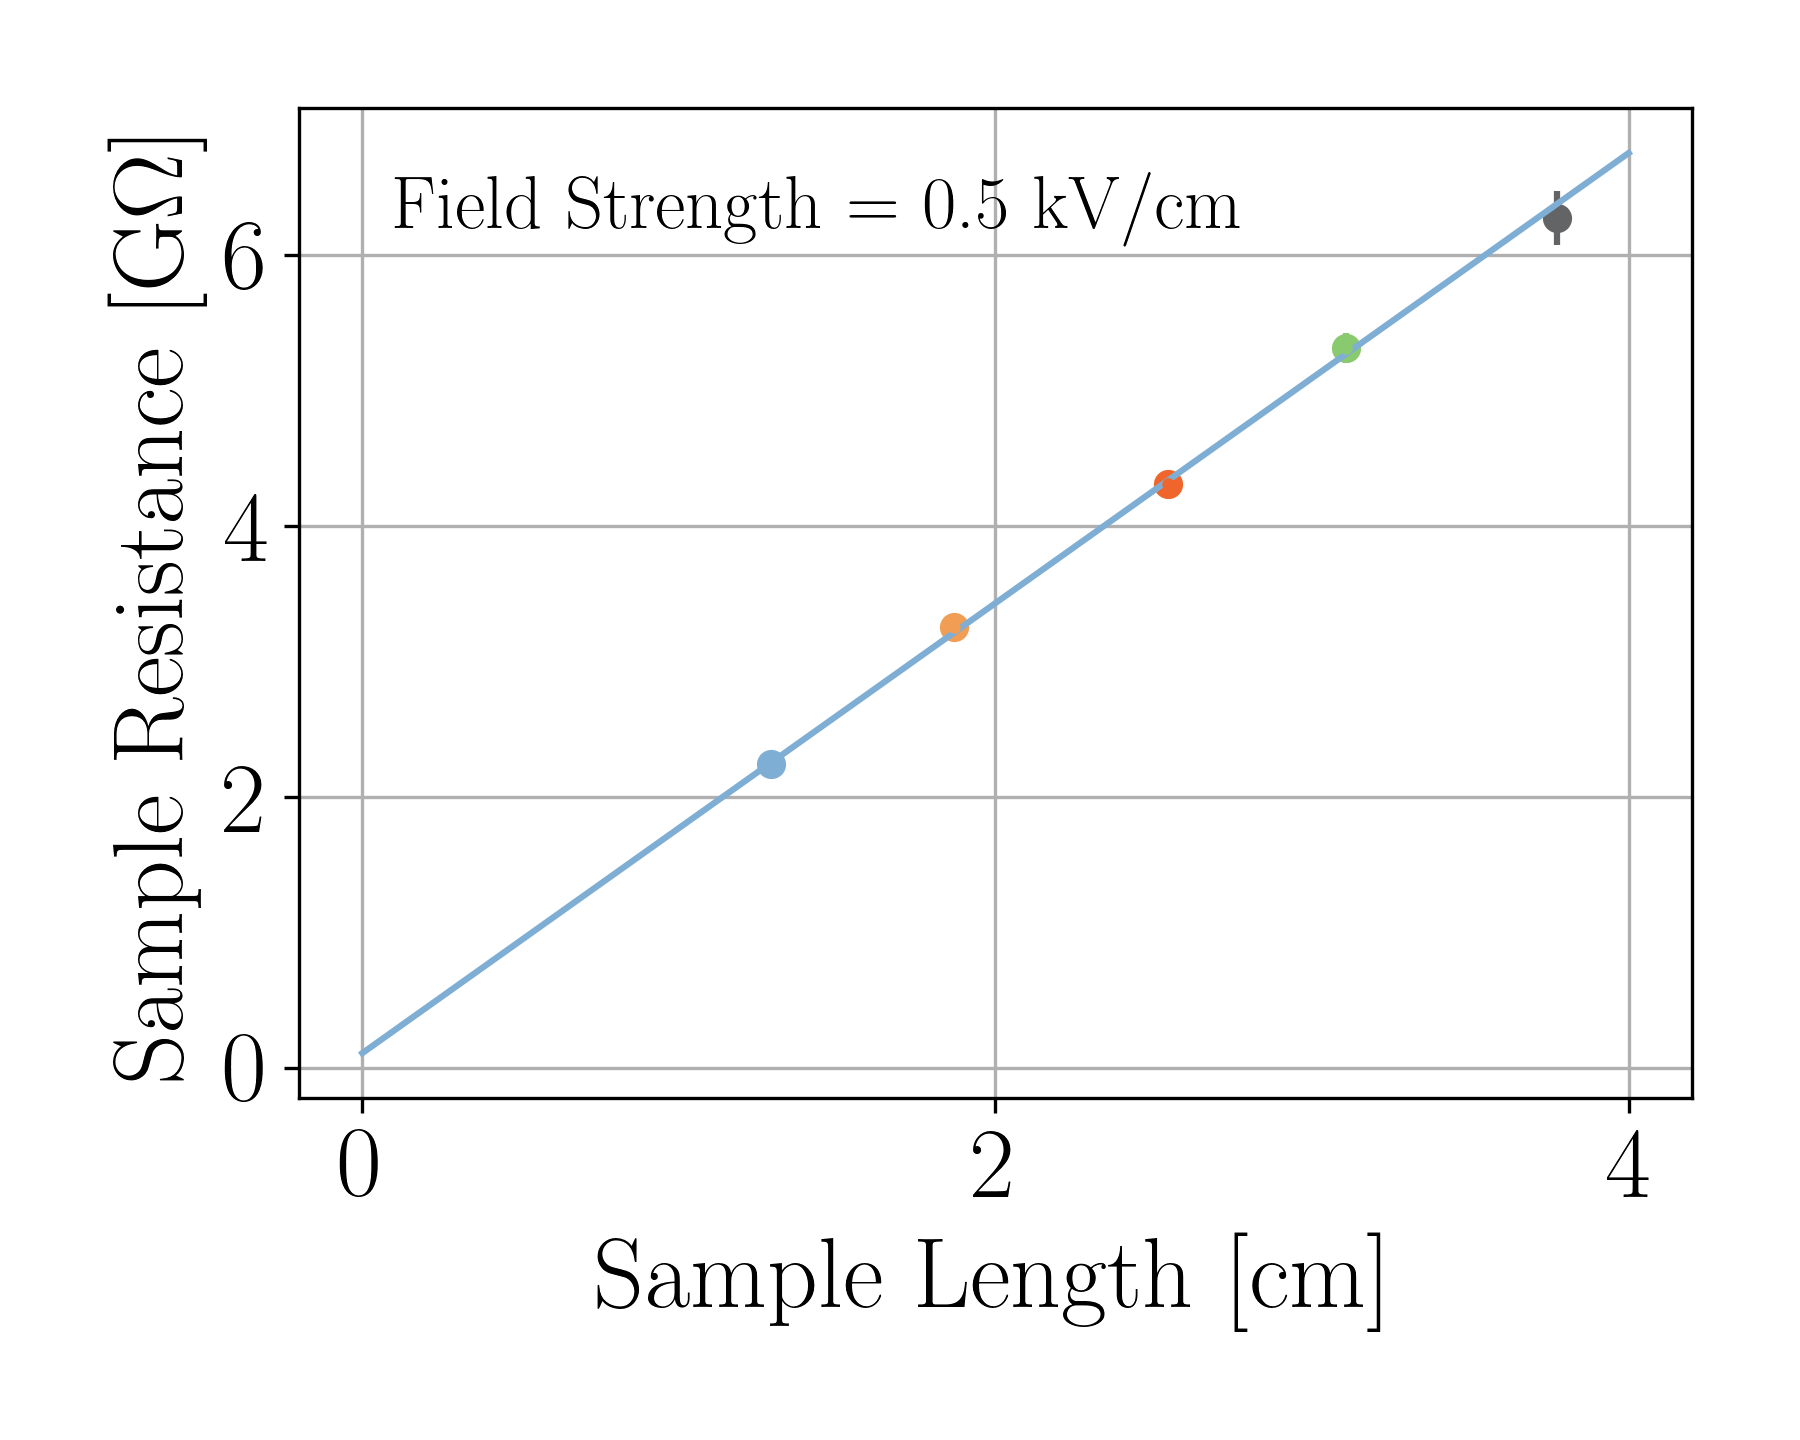
\includegraphics[width=\textwidth]{TLM_length_TLMfit.png}
		
		\vspace*{-\baselineskip} \hspace{1em} (a)
	\end{center}
\end{subfigure}
\begin{subfigure}[c]{0.32\textheight}
	\begin{center}
		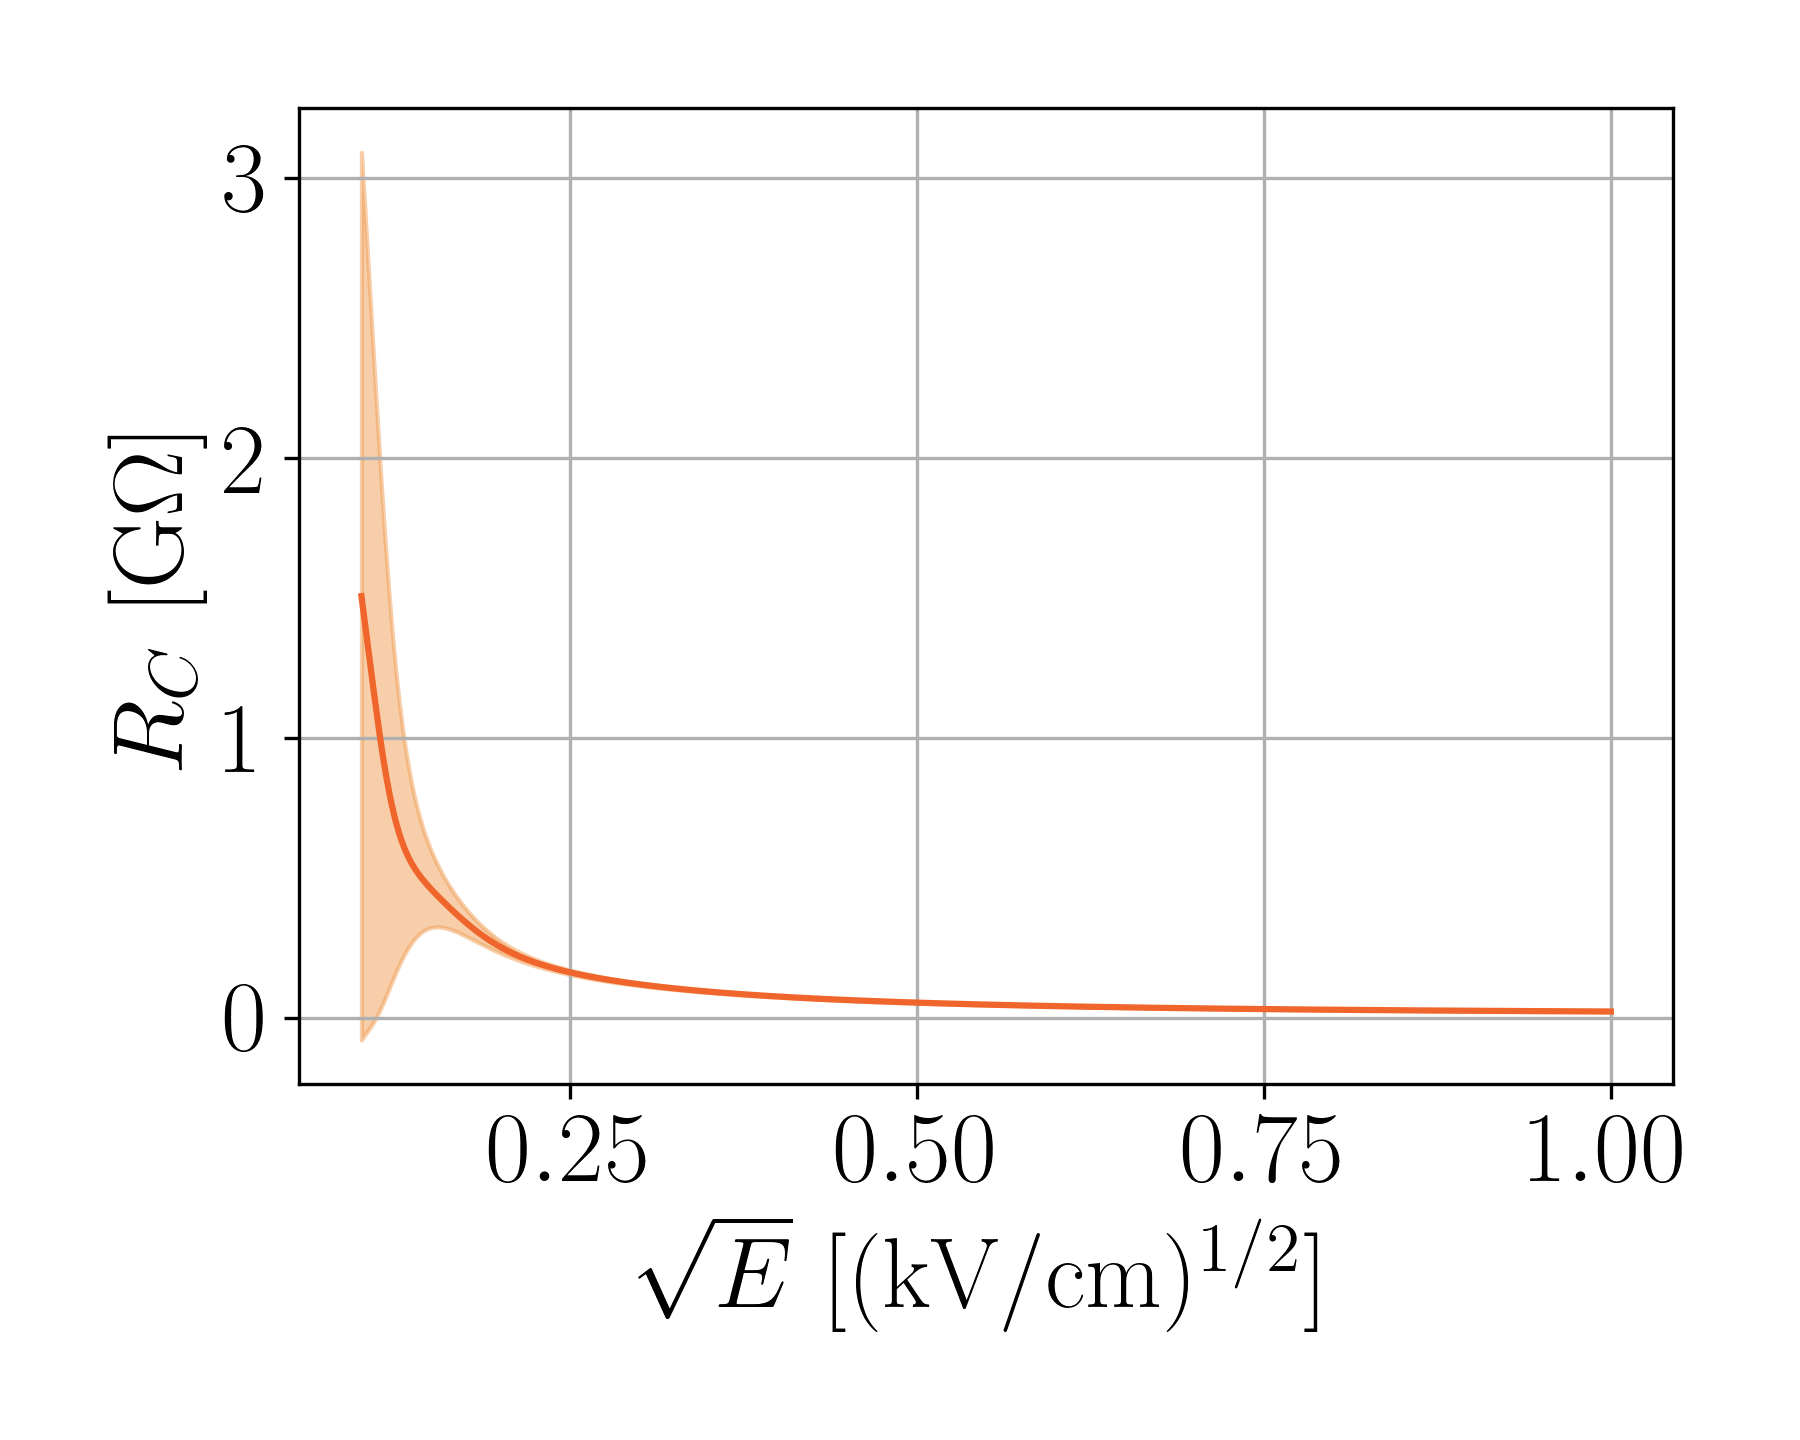
\includegraphics[width=\textwidth]{TLM_length_contactRes.png}
		
		\vspace*{-\baselineskip} \hspace{2em} (b)
	\end{center}
\end{subfigure}
\caption{(a) For a single value of the electric field, the model-fit values follow a very linear trend as a function of contact-to-contact distance.  The y-intercept of the linear fit corresponds to the resistance of both contacts. (b) The measured contact resistance as a function of the electric field (central dark orange line) and the associated uncertainty band in light orange. The associated uncertainty is obtained from the variance of the intercept parameter in the TLM fit.} 
\label{fig:TLM_length_contactRes}
\end{figure}

\todo{Increase size of this figure after clean up}


\subsection{Contact Overlap}
\label{sec:contactOverlap}

The contact resistance measured in section~\ref{sec:transLine} is in principle a function of the geometry of the contact patch between the copper and {\DR}.  The nature of this dependence is non-linear, as the current density through the copper-{\DR} interface is much higher close to the inner edges than on the outside of the sample.

In order to test the dependence on the contact size (i.e., overlap between the {\DR} and copper strip), here onward referred to as contact overlap, a  sample with an $\approx 1$\," wide copper strip on either side of the {\DR} is used to measure the dependence on the contact overlap.  The sample is tested through a voltage range of (0--5)\,kV in an L\ch{N2} bath, as in the previous section.  After each test, the sample is allowed to warm to room temperature and then the contact width is reduced by cutting the {\DR} sample by a small amount on the outer side.  This method preserves the geometry and material features of the {\DR} sample while changing only the amount of copper-{\DR} interface through which current is allowed to flow.


\begin{figure}[htb]
\centering
\begin{subfigure}[c]{0.32\textheight}
	\begin{center}
		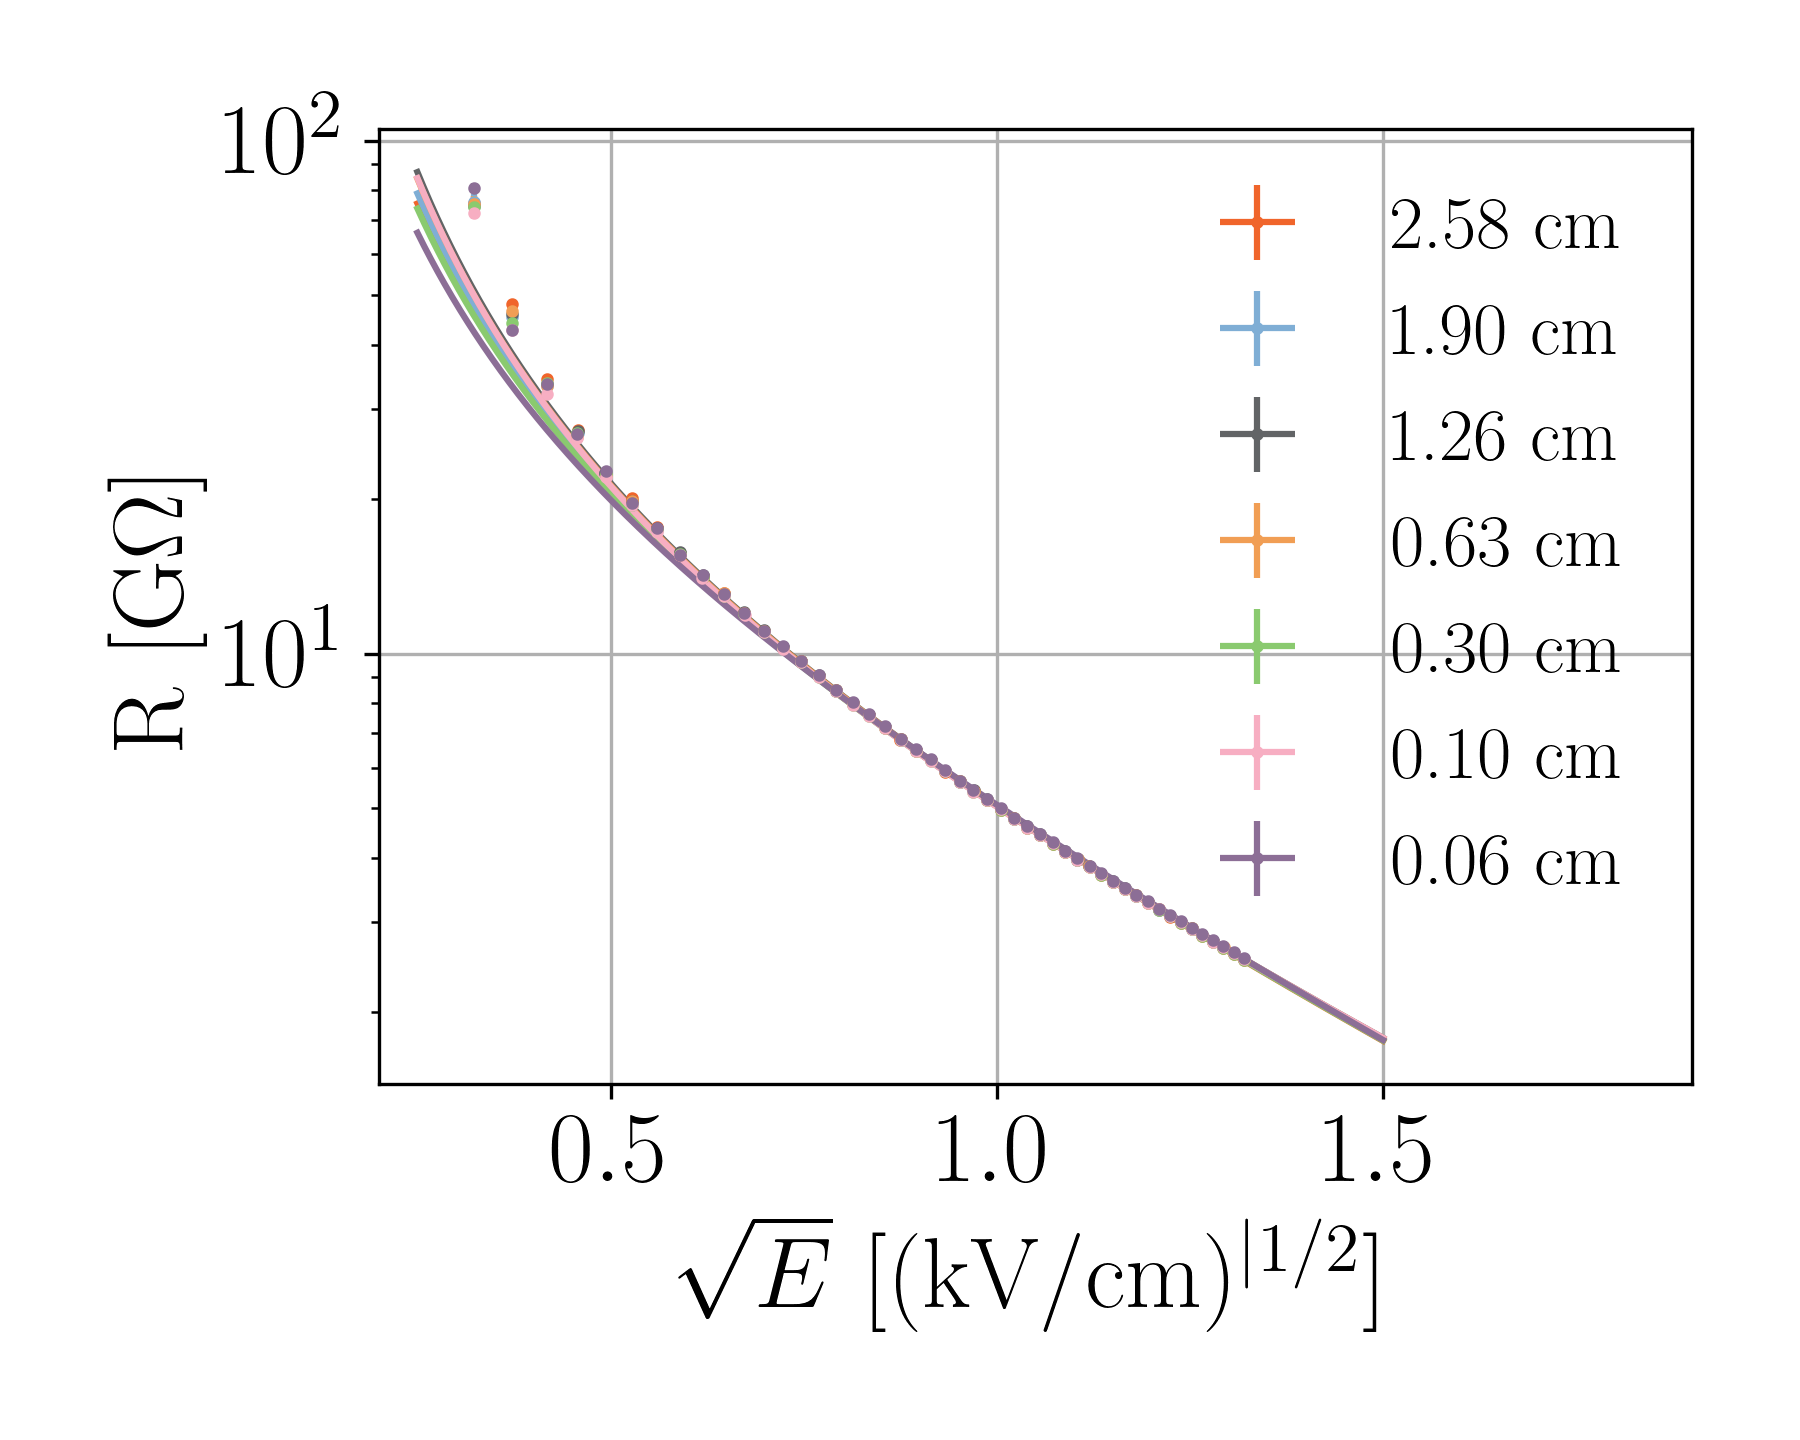
\includegraphics[width=\textwidth]{TLM_contact_resistance.png}
		
		\vspace*{-\baselineskip} \hspace{1em} (a)
	\end{center}
\end{subfigure}
\begin{subfigure}[c]{0.32\textheight}
	\begin{center}
		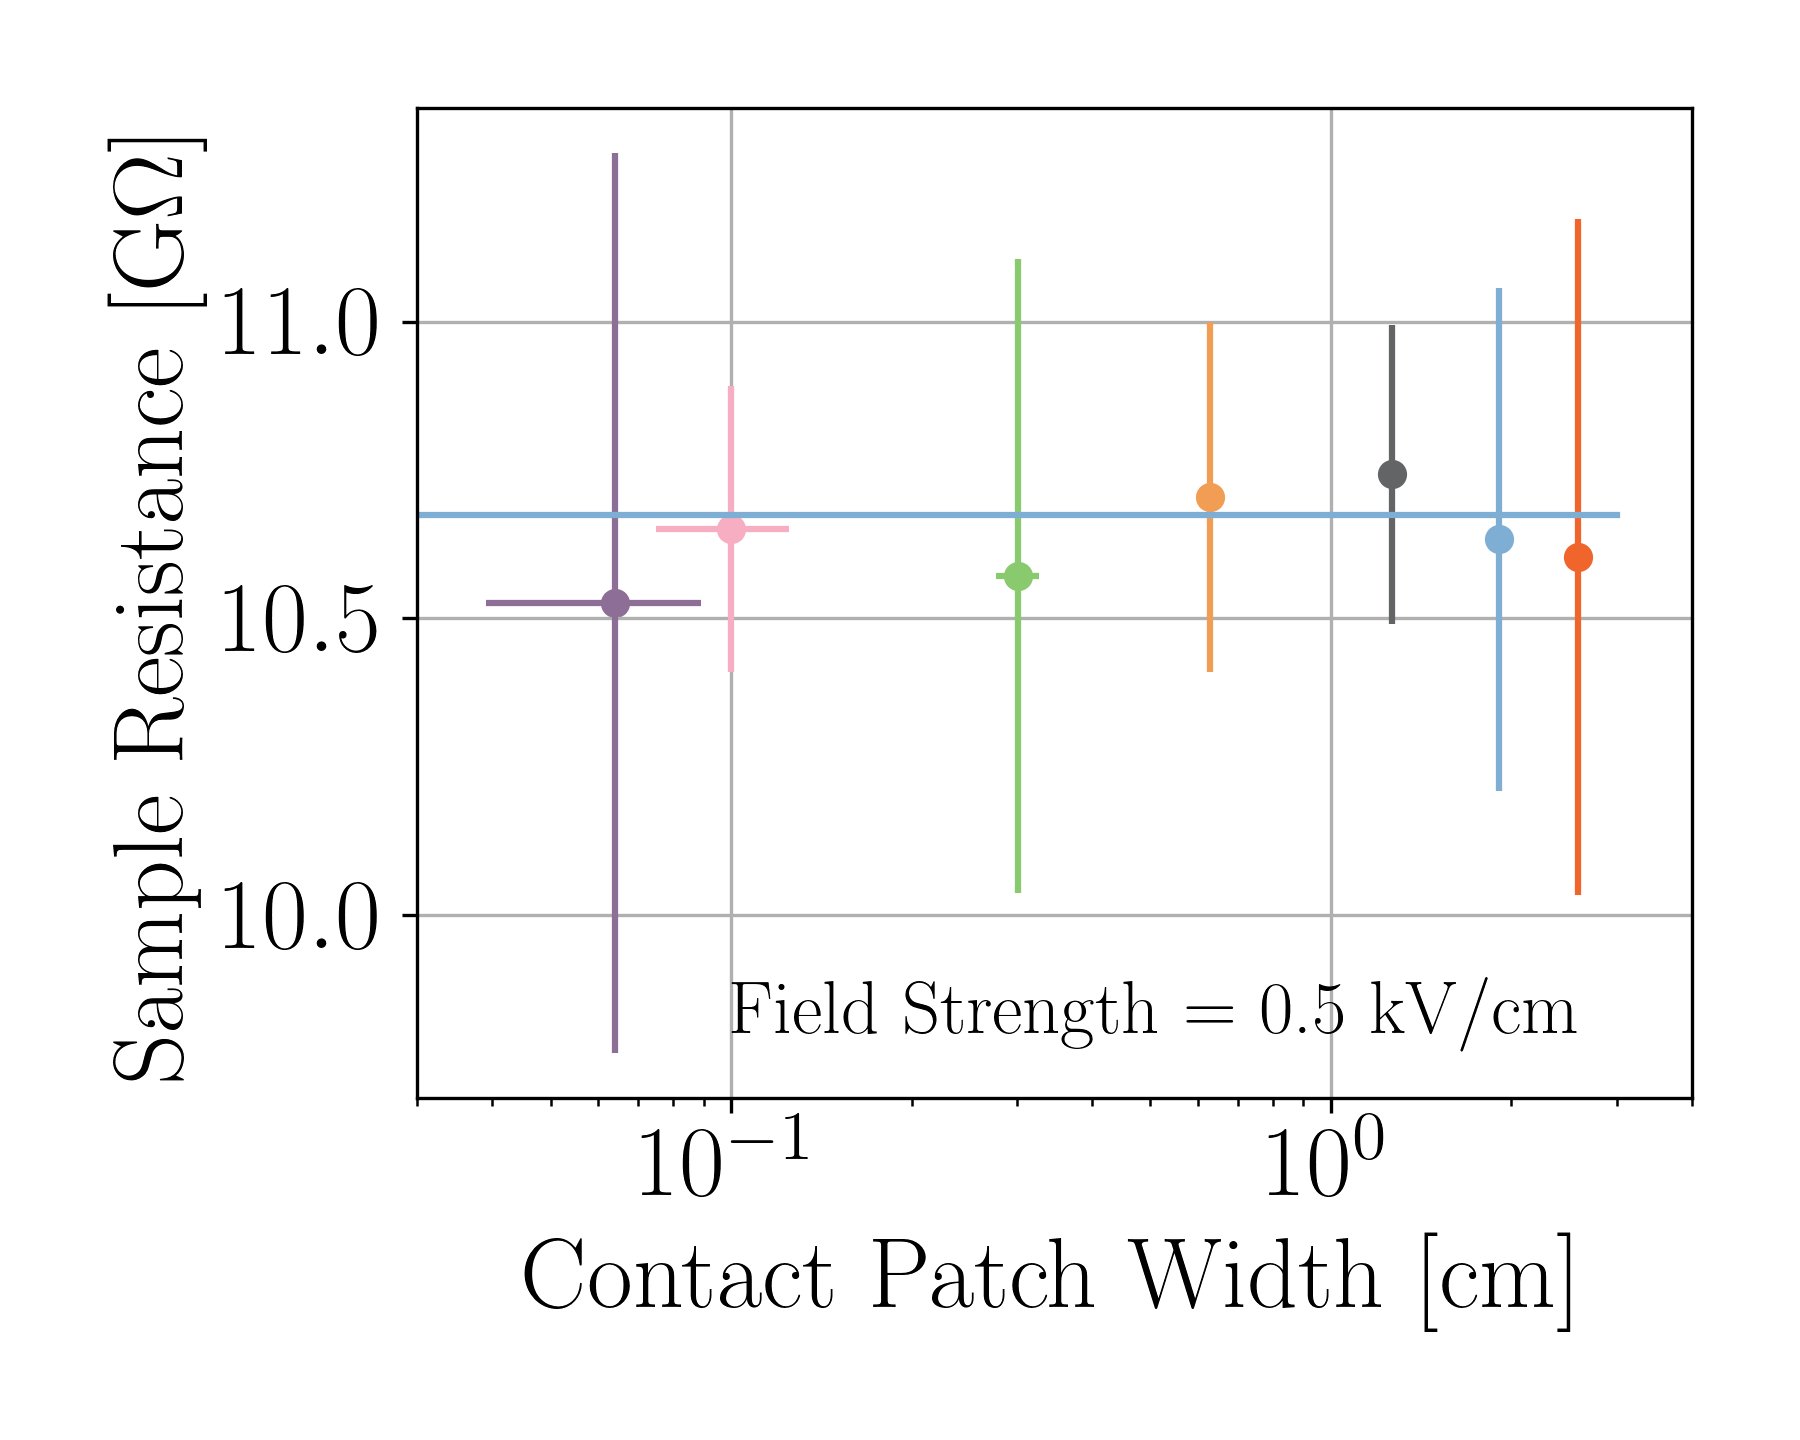
\includegraphics[width=\textwidth]{TLM_contact_fit.png}
		
		\vspace*{-\baselineskip} \hspace{2em} (b)
	\end{center}
\end{subfigure}
\caption{(a) The measured resistances of the different samples.  These values are constructed in the same manner as in Figure~\ref{fig:TLM_length_I_and_R}.  The measured values are nearly identical from sample to sample. (b) For a given value of the electric field (500\,V/cm), the measured resistance is shown to have very weak dependence upon the width of the contact for the range of (0.06--2.58)\,".} 
\label{fig:TLM_contact_contactRes}
\end{figure}

The result of this measurement, shown in Figure~\ref{fig:TLM_contact_contactRes}, is a very weak dependence on contact width.  This is consistent with the findings in section~\ref{sec:transLine}, which indicate that the overall resistance of the sample is dominated by the {\DR} material itself, and not the contacting method used.  It is also possible that, if a strong dependence on this aspect of the sample exists, it is observable only on scales much smaller than are achievable by our methods (down to $\approx 0.5$ mm).  A TPC using a field cage of this design would typically have 1 cm of contact overlap in the field shaping elements.


\subsection{Time dependence, and resistivity degradation}
\label{resdecayfit}

\todo{Frankie this is the aging bit; too old for you}

As we explored higher electric fields, for longer periods of time, we noticed the sheet resistance decreases with time. We try to to characterize this time-dependence using an empirical model of an exponential decay, introducing $\tau$, the decay constant. Notice that this behaviour dependence on the electric field and so $\tau$ is actually a function of the electric field.

During the cooling of the system ($\approx3$\,hrs) this effect is negligible, both because the time scale and as it is less profound in lower voltages (the system is set to $\approx5$\,kV \RI{(Zach please check this number)} during the cooling of it). However, for higher electric fields and longer periods of time, we need to better account for the time dependence in addition to the temperature dependence, in order to quantify the resistance as a function of the applied electric-field. Thus, we simultaneously fit the time, temperature and electric-field using
we began to notice that fits with the above model were worse and worse. Visual inspection of sheet resistance and temperature curves such as those in Figure\ref{fig:43750} forced us to model a decreasing sheet resistance with time, independent of temperature, in order to fit. As a very simple model, we posit that this behavior is characterized by exponential sheet resistance decay caused by breakdown at such high electric field. 

This is not visible in the cooldown curve because the voltage was is necessarily low before the sample is fully submerged, and thus no resistive decay with time is observed during that period, leading to a good fit with the previous method. However, at higher electric field, we can no longer expect that the resistivity is constant in time, even with arbitrarily constant temperature. Thus for a particular electric field sub-run, in order to isolate and separate these effects, we need to eliminate the time-varying temperature dependence from the time-varying electric-field decay. We model both of these behaviors as 

\RI{Zach - Im not sure you discussed the "decay" at this point, I actually think it would be good not to, keep the focus here on the temperature only, I think the next step would be to explain how we "integrate-out" the temperature, which allows us to get the E-field dependency}


\begin{equation}
	R_{s}^{meas}(t,T)=R_s\exp\bigg(\sqrt{\frac{T_0}{T}}- \frac{t}{\tau}\bigg)=R_s(t)\exp\bigg(\sqrt{\frac{T_0}{T}}\bigg),
\end{equation}
where $t$ is the measured time and $\tau$ is the time constant of the decay at a particular electric field. In addition to better account for any tim-varying temperature depandance we modufy eq~\ref{eq:Tdep} to
\begin{equation}
	R_{s}^{meas}(t,T)=R_{s}^{meas}(t,T')\exp\bigg(-\sqrt{\frac{T_0}{T'}}+\sqrt{\frac{T_0}{T}}\bigg).
\end{equation}
where again, we choose $T=95$\,K s our reference temperature.

Now with inputs of the temperature as a function of time, $T(t)$ and the resistance as a function of time, $R_{s}^{meas}(t,T)$, we can fit for our three fit constants $R_s,T_0,$ and $\tau$.
Also, our new temperature "normalization" for sheet resistance curves taken at different temperatures is :
\begin{equation}
R_{s}^{meas}(t,T)=R_{s}^{meas}(t,T')\exp\bigg(-\sqrt{\frac{T_0}{T'}}+\sqrt{\frac{T_0}{T}}\bigg).
\end{equation}
where again, we compare all curves at the choice of constant $T=95K$.


\subsubsection{Bootstrapping and Time Constants}
In order to analyze the resistive decay of the sample during a time interval at a given electric field, the quantity of interest is the time constant, $\tau$, which we extract by fitting the sample's sheet resistance as described in section~\ref{resdecayfit}. However, the uncertainties on the fit parameters, specifically $\tau$, are not the relevant uncertainties for a ``measurement'' of $\tau$, as they are suppressed by the Poisson error, while the number of "measurements" of $\tau$ is certainly not this high\RI{do you want to give numbers here}. In order to understand the true uncertainties of our measurement, we make the assumption of constant exponential resistive decay throughout the entire time interval \RI{Zach maybe here add allowing us to use a sequential bootstrapping bla bla}. With this assumption, we remove the temperature dependence across the whole multi-hour sample according to the same methods described in section~\ref{resdecayfit}. With this multi-hour temperature-normalized sample, we take each successive hour-long interval to comprise an independent sample with a corresponding measurement of $\tau$. We fit each interval to an exponential, recording the resulting $\tau$, and this results in an independent measurement of $\tau$'s for each hour of the full sample with a resultant measurement uncertainty. We can see the resulting $\tau$ measurements in Figure~\ref{fig:invtaulog}.

\begin{figure}
	\begin{center}
		
		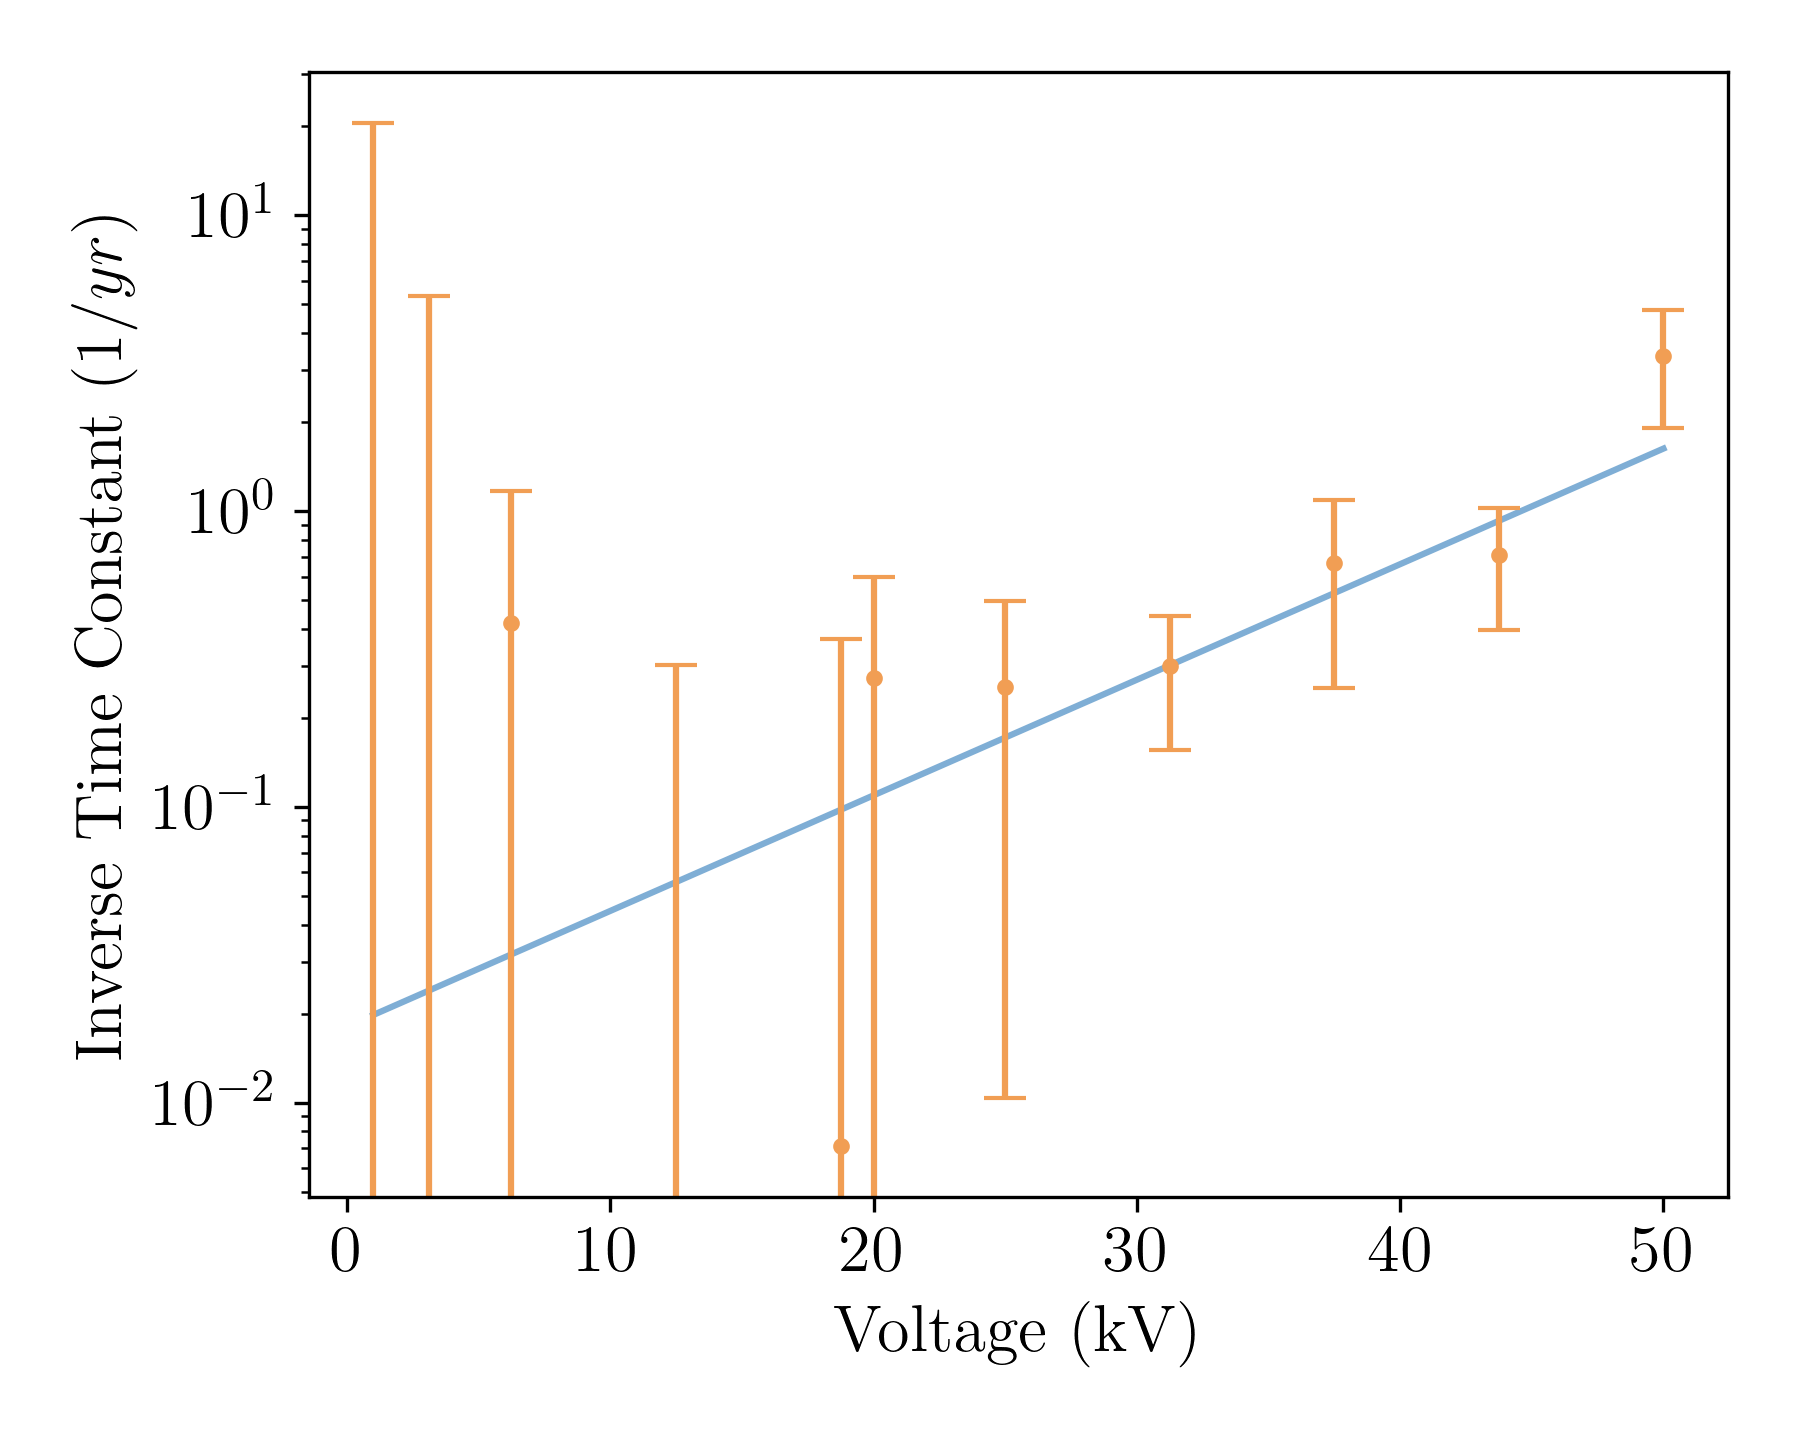
\includegraphics[width=0.75\linewidth]{tau.png}
		\caption{Inverse decay constants as a function of voltage. Runs with less than a 24 hour period are suppressed.} 
		\label{fig:invtaulog}
	\end{center}
	
\end{figure}




\subsubsection{Long Term Results \RI{change title}}
\label{sec:long_term_results}
Now, we return to our original goal for this set of runs, to ascertain the viability of DR8 as a material for long term use in liquid Argon at the DUNE near detector. 

Our first point to verify is the resistive properties of this material in liquid argon; specifically, does this material meet the resistive demands from DUNE ND and other TPCs? For DUNE ND specifically, the lower bound on the required resistivity comes from the heat dissipation, while the necessity of dissipating the deposited charge in the system sets a maximum allowable resistivity???

\begin{figure}
	\begin{center}
		
		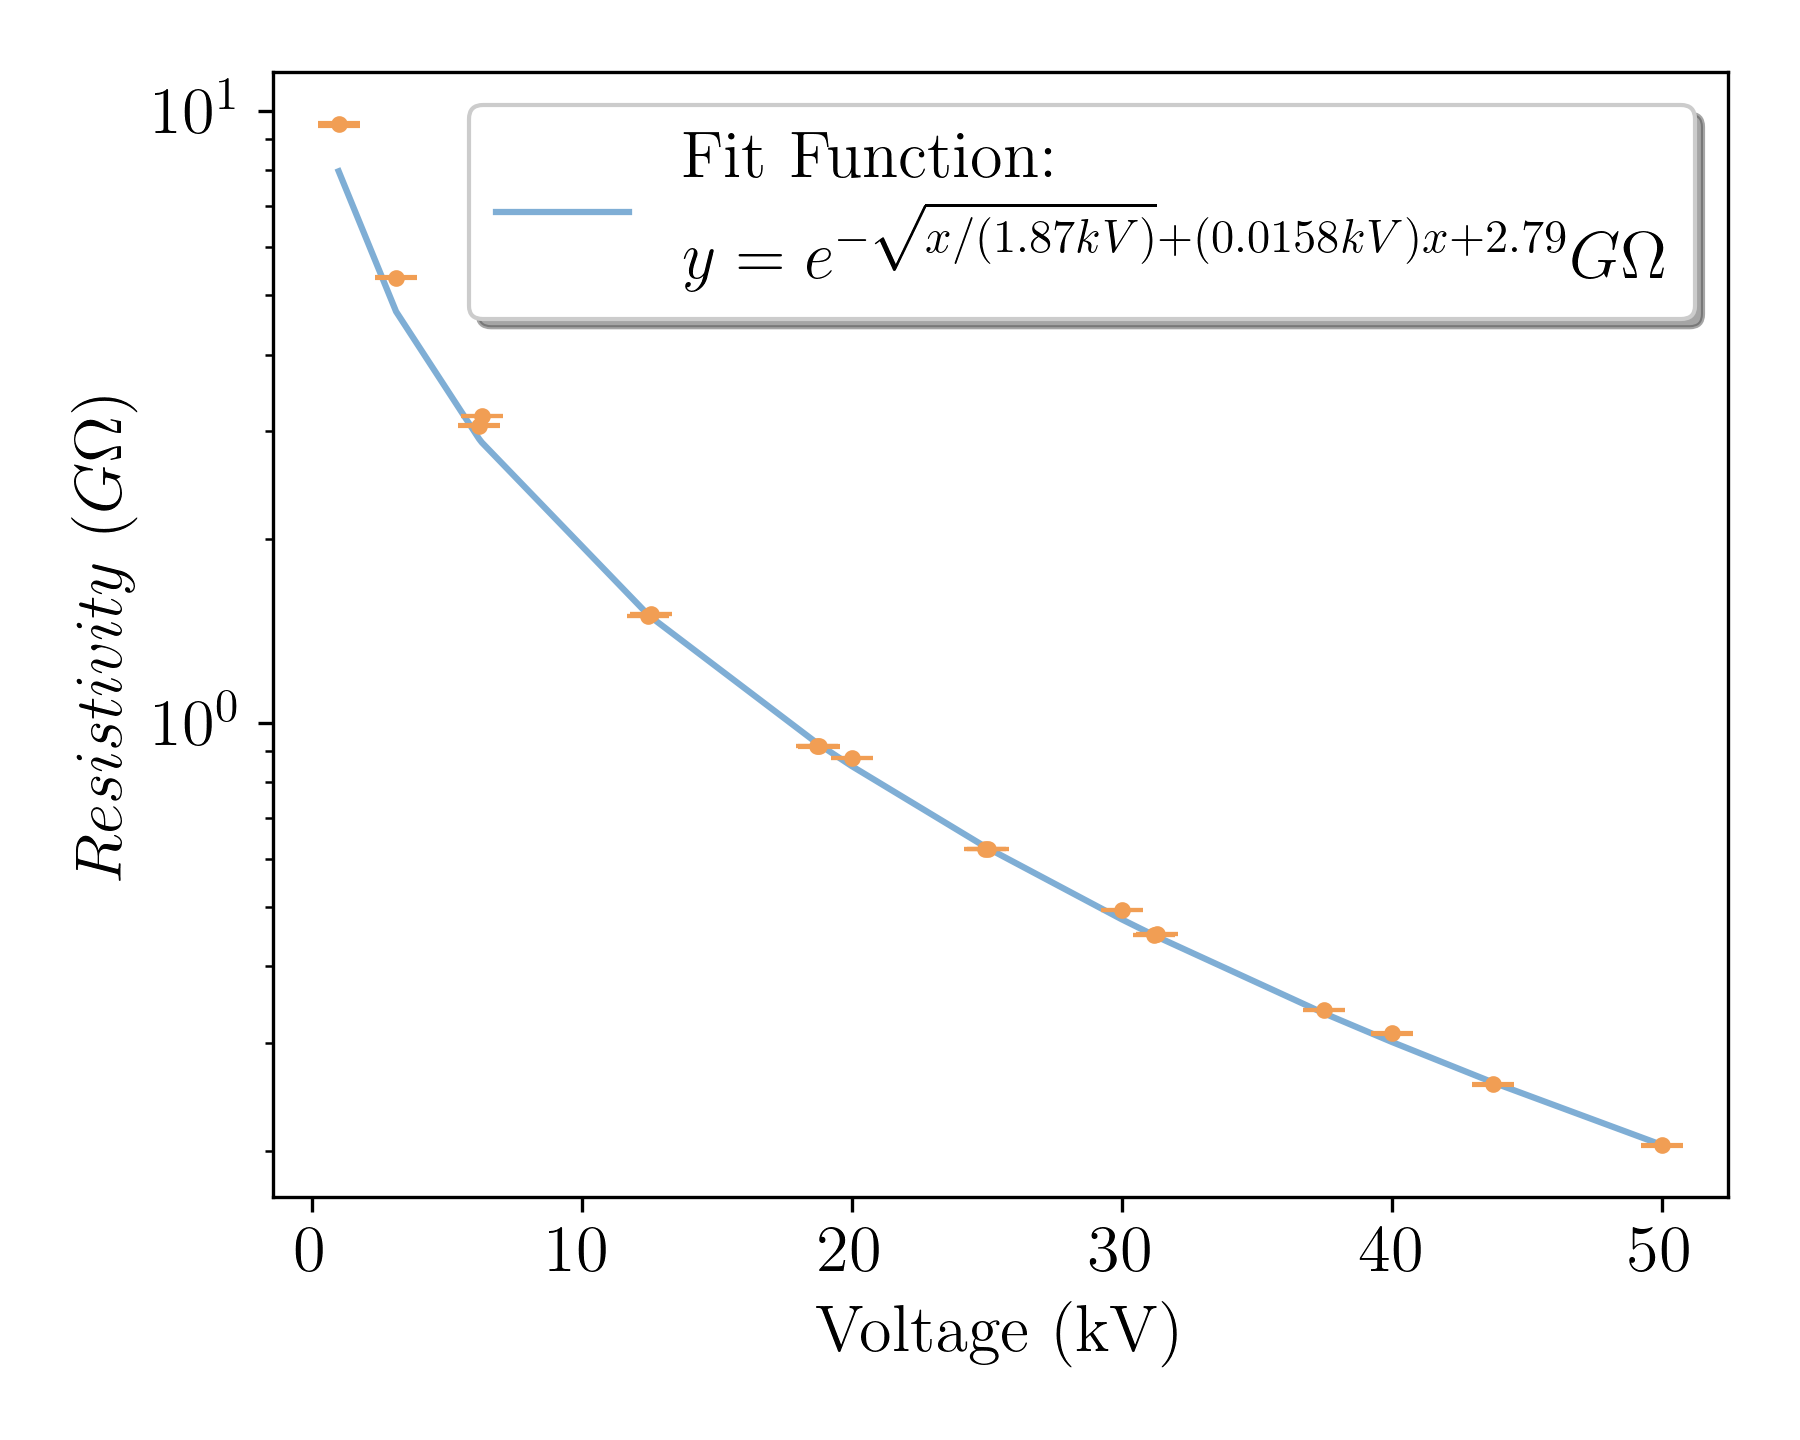
\includegraphics[width=0.75\linewidth]{Efield_Z.png}
		\caption{Resistance as a function of the voltage of the subrun, with fit to the Hopping model described previously.\RI{no need for the words fit function, or for the function itself, one is enough. I guess we can leave the function}} 
		\label{fig:resvsvol}
	\end{center}
\end{figure}


Second, at what electric field scale does this material begin to decay? Our measurements are consistent with zero decay below 2000V/cm at the 1-sigma level, although increasing measurement uncertainty at lower E-fields does cloud the measurement of the decay there. However, from Figure~\ref{fig:invtaulog}, we can see a clear trend of increasing decay as the E-field increases.


\todo{Kendall: Does Dan have this data, if not him then need Zach. Add a new subfigure--  one clear example how the drift looks, see how it is changing. Then, plo  field str not voltage }

Finally, what can we say about the longevity of this material in operating conditions at DUNE ND?
As shown in Figure~\ref{fig:resvsvol}, the scaling decay of the sample with voltage is well modeled by the  decay rate exponentially increasing with voltage. At 6.25 kV, the voltage corresponding to 500 V/cm, the time constant is consistent with infinitely long at the 1-sigma level and predicted by this simple model to be at least on the order of decades. Thus, from a longevity point-of-view, our measurements discern no problem with using this material in DUNE-ND.


\section{Discussion and Conclusions}
\label{sec:sum}

\todo{Confirm discussion of Hopping model is sufficiently covered by Fig 11}

summary

\section{Acknowledgment} 



\clearpage
% ========================================================================
% bibliography
% ========================================================================
%\printbibliography
\bibliographystyle{JHEP}
\bibliography{DR8Bib}

\end{document}